\documentclass[11pt,a4paper]{article}

% ----------------------------------------------------------------------
%  Acquisition-parameter sweep review, 2026-08-17 -> 2026-08-19
%  Companion documentation log to report/main.tex.
%  No LaTeX toolchain on the acquisition machine -- compile on Overleaf
%  (upload the whole report/ folder) or with a local TeX Live:
%      latexmk -pdf acquisition_sweep_log.tex
% ----------------------------------------------------------------------
\usepackage[utf8]{inputenc}
\usepackage[T1]{fontenc}
\usepackage{lmodern}
\usepackage[margin=2.4cm]{geometry}
\usepackage{graphicx}
\usepackage{booktabs}
\usepackage{amsmath}
\usepackage{siunitx}
\usepackage{xcolor}
\usepackage{caption}
\usepackage{subcaption}
\usepackage{enumitem}
\usepackage{microtype}
\usepackage{longtable}
\usepackage{multirow}
\usepackage[hidelinks,colorlinks=true,linkcolor=blue!55!black,citecolor=blue!55!black,urlcolor=blue!55!black]{hyperref}

\graphicspath{{figures/}}
\captionsetup{font=small,labelfont=bf}
\setlist{itemsep=2pt,topsep=3pt}

\newcommand{\good}[1]{\textcolor{green!45!black}{\textbf{#1}}}
\newcommand{\caveat}[1]{\textcolor{orange!75!black}{\textbf{#1}}}
\newcommand{\bad}[1]{\textcolor{red!65!black}{\textbf{#1}}}
\sisetup{detect-weight=true,detect-family=true}

\title{\vspace{-1.5em}\textbf{Acquisition-parameter sweeps of August 2026:\\
what the phantom says, what the probes say,\\ and why the heart still says nothing}\\[0.4em]
\large A documentation log for the \texttt{shearWaveProcessing} / \texttt{SWI} projects}
\author{TU Eindhoven --- Shear-wave elastography}
\date{19--20 August 2026}

\begin{document}
\maketitle

\begin{abstract}
\noindent
This is a working log, not a paper. It records what was done between 17 and 20 August 2026 to test the
acquisition recommendation of the previous report (\texttt{report/main.tex}): that the in-vivo cardiac
ARF shear-wave measurement fails because the push is too weak, and that a larger push aperture plus a
longer push pulse should fix it. Four questions were asked of four new datasets. The short version is:
(i) the processing pipeline reproduces the earlier high-quality phantom space-time plots exactly;
(ii) the new phantom sweep reproduces the earlier parameter ranking --- but only when apertures are
compared at equal \emph{transmit voltage}, and the ranking \emph{inverts} when they are compared at
equal \emph{acoustic output}, which is what the safety limit actually constrains; (iii) the TU/e and
MUMC S5-1 probes are indistinguishable, so the transducer is not the problem; and (iv) neither new
in-vivo configuration produces a shear wave that beats its own no-push control. A substantial part of
the work was not analysis at all but debugging: every acquisition made after 7 August was being
reconstructed from the raw RF with the wrong sample stride, which silently destroyed the tracking data
and had already produced one round of wrong conclusions. That bug, its diagnosis and its fix are
documented here in full because it will otherwise be re-hit.
All hydrophone sessions were then re-analysed together on one set of conventions
(\S\ref{sec:safety}), which matters because the whole aperture argument turns on the acoustic-output
axis: the 41-element push \emph{has} been measured directly (2026-08-17), and the resulting limit is
\SI{32}{\volt}, not the \SI{35}{\volt} the earlier extrapolation suggested. Finally
(\S\ref{sec:trend}) the aperture trend is extended down to 21 elements using data that was already
in hand, which shows the optimum is not at the smallest aperture but near 41.
\end{abstract}

\tableofcontents

% ======================================================================
\section{Scope, and how to read this log}
% ======================================================================
The previous report established, on a CIRS phantom and on the published Caenen pig dataset, that the
processing pipeline recovers a clean symmetric ARF shear wave, and that our own transthoracic in-vivo
recordings do not contain one. It attributed that failure to the acquisition --- specifically to an
underpowered, deep, loosely-focused push --- and recommended \textbf{61 push elements and a
$\sim$\SI{800}{\micro\second} pulse} on the basis of a one-at-a-time phantom parameter sweep
(11 configurations $\times$ \{20, 30\}\,V) in which push aperture was by far the dominant lever.

Between 17 and 18 August three new datasets were acquired to test that recommendation, and a hydrophone
campaign (documented separately in \texttt{HydrophoneSafety\_Notes.md}) had in the meantime established
what the sequences are actually \emph{allowed} to transmit. This log covers the analysis of those
datasets, in the order the questions were posed:

\begin{enumerate}[label=\textbf{Q\arabic*.}]
  \item Can the high-quality phantom space-time plots of the report (the clear symmetric ``V'') be
        reproduced from the raw data?
  \item Do the results of the \texttt{2026\_08\_17 Phantom sweep elements cycles TXvoltage} dataset
        agree with the report? (Deliverable: two $5\times3$ grids --- 2 pulse lengths, 3 element
        counts, 5 transmit voltages.)
  \item How does \texttt{2026\_08\_18 TUe MUMC comparison} compare, on the same phantom, with two
        different S5-1 probes?
  \item Does the proposed change in acquisition parameters actually produce clearer shear-wave
        propagation \emph{in vivo}
        (\texttt{2026\_08\_18 Invivo cycles elements TXvoltage})?
\end{enumerate}

Section~\ref{sec:data} lists the data, Section~\ref{sec:questions} the hypotheses,
Section~\ref{sec:problems} the problems encountered (this is the longest section, and deliberately so),
Section~\ref{sec:methods} the processing and scoring, Sections~\ref{sec:q1}--\ref{sec:q4} the results,
Section~\ref{sec:crossbeat} a fifth question the data answered on its own, Section~\ref{sec:conclusions} the conclusions, and Sections~\ref{sec:recommend}--\ref{sec:next} the
recommendation and what is still open.

% ======================================================================
\section{Data sources}\label{sec:data}
% ======================================================================
All acquisitions use the S5-1 phased array (80 elements, pitch \SI{0.254}{\milli\metre}) with the
6-buffer SWI widebeam sequence; the ARF push is at \SI{2.25}{\mega\hertz}. Phantom acquisitions use the
CIRS elasticity phantom with the push focus at \SI{49.3}{\milli\metre} and PRI
\SI{270}{\micro\second} (tracking PRF \SI{3.70}{\kilo\hertz}), 10 pushes per measurement.
Table~\ref{tab:data} lists everything used here, including the two older datasets that serve as
known-good references.

\begin{table}[h]
\centering\small
\caption{Datasets used in this log. ``Reference'' datasets were acquired earlier and are known to
process correctly; they are used to validate the repair described in \S\ref{sec:bug} and to
provide a baseline. All live under
\texttt{D:\textbackslash Luuk van Knippenberg\textbackslash Claude\textbackslash MI estimation}.}
\label{tab:data}
\begin{tabular}{@{}p{4.6cm}p{2.0cm}p{2.2cm}p{6.2cm}@{}}
\toprule
\textbf{Dataset} & \textbf{Role} & \textbf{Folders} & \textbf{Content} \\
\midrule
\texttt{2026\_08\_04 .../Phantom} & reference & 8 & Push-voltage sweep 50\,$\rightarrow$\,15\,V,
41\,el / 1500\,cyc, 2 pushes each. The report's ``clean anchor''. \\
\texttt{2026\_08\_04 .../Invivo} & reference & 2 & Transthoracic PLAX septum, free-running,
24 pushes, 41\,el / 1500\,cyc at 30 and 40\,V. Has \emph{hand-drawn} M-lines. \\
\texttt{2026\_08\_04 .../Phantom parameter sweep} & reference & 22 & The 2026-08-07 one-at-a-time
sweep (pulse length, aperture, PRF) $\times$ \{20, 30\}\,V that produced the 61-element
recommendation. Acquired at \texttt{SW.endDepth}\,=\,200\,wl. \\
\midrule
\texttt{2026\_08\_17 Phantom sweep elements cycles TXvoltage} & \textbf{Q2} & 30 &
Full grid: \{41, 61, 79\} elements $\times$ \{1500, 1900\} cycles $\times$ \{20, 25, 30, 35, 40\}\,V,
10 pushes each. Same phantom, same geometry. \\
\texttt{2026\_08\_18 TUe MUMC comparison} & \textbf{Q3} & $2\times34$ &
The same 30-cell grid repeated with the TU/e and with a borrowed MUMC S5-1, on the same phantom
within \SI{45}{\minute}; plus one focused B-mode of a resolution phantom per probe. \\
\texttt{2026\_08\_18 Invivo cycles elements TXvoltage} & \textbf{Q4} & 2 &
Transthoracic PLAX septum, \textbf{R-peak triggered}, 24 pushes at \SI{20}{\hertz}:
41\,el / 1500\,cyc / 30\,V and 61\,el / 1900\,cyc / 25\,V. \\
\midrule
\texttt{S5-1\textbackslash} hydrophone, \textbf{session A} (2026-08-13/14) & safety & 7 folders &
Onda HGL-0400 + AH-2010-025 preamp, 50\,$\Omega$ scope. Focused-imaging sweep 2--20\,V; push
79\,el 2--12\,V; push 61\,el 3--8\,V; axial/lateral scans. Low voltages only (the preamp clips at
$\sim$2.2\,V into 50\,$\Omega$), so the limits were \emph{extrapolated}. No 41-element data. \\
\texttt{S5-1\textbackslash S5-1 push with and without preamp}, \textbf{session B} (2026-08-17) &
safety & 1 folder & Hydrophone straight into the 1\,M$\Omega$ scope (no preamp $\rightarrow$ no
clipping), so 15--50\,V is measured \emph{directly}. Push \textbf{41 / 61 / 79 elements},
15--50\,V, peak-optimised captures; 61-el base also 2--12\,V (overlaps session A and calibrates the
cable+scope load); \texttt{79 elements repeats\textbackslash} holds 3 consecutive firings per
capture. \\
\bottomrule
\end{tabular}
\end{table}

\paragraph{What the hydrophone campaign contributed.} The relevant result is not a number but a
constraint: the S5-1 ARF push is \textbf{$I_\mathrm{sppa.3}$-limited}, not MI-limited and not
$I_\mathrm{spta}$-limited. At each aperture's legal maximum the derated MI has only reached
1.5--1.6, while $I_\mathrm{sppa.3}$ already sits at its \SI{190}{\watt\per\square\centi\metre}
limit; $I_\mathrm{spta.3}$ stays far below \SI{720}{\milli\watt\per\square\centi\metre} because the
real duty cycle is \SI{20}{\hertz} for \SI{1.2}{\second} followed by $\geq$\,\SI{30}{\second} idle
($\approx$\,\SI{0.77}{\hertz} effective). The maximum allowed transmit voltage therefore \emph{falls}
as the aperture grows. \S\ref{sec:safety} re-derives those numbers from both sessions together;
they are the single most consequential input to this log.

% ======================================================================
\section{Research questions and hypotheses}\label{sec:questions}
% ======================================================================
\begin{description}[leftmargin=1.4em,style=nextline]
  \item[H0 (the standing hypothesis).] The in-vivo ARF shear-wave measurement fails because the push
  is too weak to generate a detectable wave in a moving myocardium; it is acquisition-limited, not
  processing-limited.
  \item[H1 (Q1).] The pipeline is sound and the report's phantom figures are reproducible end-to-end
  from the raw data, not only as stored plots. \emph{Purpose: a positive control, so that any negative
  result on the new data can be attributed to the data.}
  \item[H2 (Q2).] Increasing the push aperture (41\,$\rightarrow$\,61\,$\rightarrow$\,79 elements) and
  the push pulse length (1500\,$\rightarrow$\,1900 cycles) improves shear-wave quality monotonically,
  and the improvement is largest at low transmit voltage (the low-SNR regime that matters in vivo).
  \item[H3 (Q3).] If the TU/e S5-1 has degraded --- a live suspicion, and the reason a second probe was
  borrowed --- the MUMC probe will produce visibly better waves on the same phantom.
  \item[H4 (Q4).] With the recommended settings (61 elements, 1900 cycles) the in-vivo space-time will
  show a clearer, more symmetric wavefront emerging from the push origin than the old
  41-element / 1500-cycle acquisition, and will beat its own no-push control.
\end{description}

\begin{description}[leftmargin=1.4em,style=nextline]
  \item[H5 (added 2026-08-20).] If a smaller aperture is better at fixed acoustic output, the trend
  should continue below 41 elements --- unless the output itself becomes unreachable first, in which
  case there is an optimum. \S\ref{sec:trend} tests this against the 21-element arm of the
  2026-08-07 sweep.
\end{description}

An implicit sixth question runs underneath all of them and is answered in \S\ref{sec:isosafety}:
\emph{given that we are safety-limited, which parameter combination should we actually use?} The
previous recommendation was derived by comparing apertures at matched transmit voltage. That comparison
is only the right one if voltage is the constraint. It is not.

% ======================================================================
\section{Problems encountered}\label{sec:problems}
% ======================================================================
This section is longer than the results sections. That is an honest reflection of where the time went.

% ----------------------------------------------------------------------
\subsection{The buffer-2 receive-layout bug (blocking; invalidated a full round of analysis)}
\label{sec:bug}
% ----------------------------------------------------------------------
\paragraph{Symptom.} Processed with the settled recipes, \emph{none} of the 2026-08-17 measurements
showed a shear wave --- not at 40\,V, not at 79 elements, not at any combination. Mirror-symmetry
scores sat at 0.04--0.34 where the 2026-08-07 sweep, at the \emph{identical} configuration
(79\,el / 1900\,cyc / 30\,V), scored 0.92--0.95. An earlier analysis round (the
\texttt{safety\_grids/} figures dated 2026-08-18) had already been produced from this data and showed
the same thing, which would have supported the conclusion ``the new acquisition failed''.

\paragraph{Diagnosis.} Three checks localised it quickly:
\begin{enumerate}
  \item The B-mode buffers (1, 3, 4, 5) looked completely normal --- same phantom, same depth, same
  bright bottom reflector as the reference datasets. So the probe, the coupling and the target were
  fine.
  \item The buffer-2 (tracking) frames did \emph{not}: the image content sat at the wrong depth, and
  the reference block sat at a different wrong depth again.
  \item The decisive number: \textbf{frame-to-frame speckle correlation near the push focus was
  0.40} (alternating between $\sim$1.0 and $\sim$0.02), against \textbf{0.98} on the 2026-08-07 data.
  Phase-based (Loupas) displacement estimation cannot survive that.
\end{enumerate}

\paragraph{Root cause.} \texttt{make\_combined\_data.m} merges the runtime parameters
(\texttt{AcquisitionParametersAndECG.mat}) with a \emph{base config} that supplies the constant
structs, including \texttt{Receive} --- the map from raw RF samples to acquisitions. For a 10-push
phantom run it auto-selects
\texttt{PhantomSweep/BaseConfig\_10frames\_<cyc>cycles\_<el>elements\_<pri>PRI.mat}. Those base configs
were recorded during the 2026-08-07 campaign with \texttt{SW.endDepth}\,=\,200 wavelengths
(\texttt{maxAcqLength}\,=\,262), giving \textbf{2688 samples} per buffer-2 acquisition. Every
acquisition from 2026-08-17 onwards was made with \texttt{SW.endDepth}\,=\,300
(\texttt{maxAcqLength}\,=\,392) $\rightarrow$ \textbf{3968 samples}.

\good{Only buffer 2 follows \texttt{SW.endDepth}}; the B-mode buffers are fixed full-depth. That is
exactly why the failure was so hard to see: the images that a human looks at were all correct, while
each successive tracking acquisition was read \num{1280} samples further into the wrong part of the
buffer, wrapping and aliasing across the frame.

\paragraph{Fix.} \texttt{scripts/fix\_buffer2\_receive.py} recomputes the layout from the runtime
parameters the way Verasonics does,
\begin{equation}
n_\mathrm{samp} = 128 \left\lceil \frac{2\,\cdot\,\texttt{maxAcqLength}\,\cdot\,
\texttt{samplesPerWave}}{128} \right\rceil ,
\qquad
\texttt{startSample}_k = 1 + (\texttt{acqNum}_k-1)\, n_\mathrm{samp},
\end{equation}
and rewrites \texttt{startSample}, \texttt{endSample} and \texttt{endDepth} in place in the
(v7.3/HDF5) \texttt{CombinedData.mat}.

\paragraph{Validation.} The rule reports \emph{``already correct''} for all 30 known-good reference
folders --- 8 from 2026-08-04 (which are at \texttt{endDepth} 300, 3968 samples) and 22 from
2026-08-07 (at 200, 2688 samples), i.e.\ it reproduces \emph{both} historical layouts --- and
\emph{``needs fix''} for all 30 folders of the new sweep. After repair, correlation returns to 0.98 and
the symmetric V reappears (Figure~\ref{fig:bug}). All 100 affected folders (30 phantom + 68 probe
comparison + 2 in-vivo) were repaired and re-beamformed.

\paragraph{Prevention.} The check is now folded into
\texttt{swp.acquisition.combined.ensure\_combined\_data} as
\texttt{repair\_buffer2\_receive()}, so it runs on every build and a mismatched base config can no
longer pass silently. \caveat{Anything computed from the 2026-08-17 or 2026-08-18 data before
2026-08-19 must be discarded}, including \texttt{safety\_grids/} and \texttt{pulse\_variance.*} in the
2026-08-17 folder.

\begin{figure}[t]
\centering
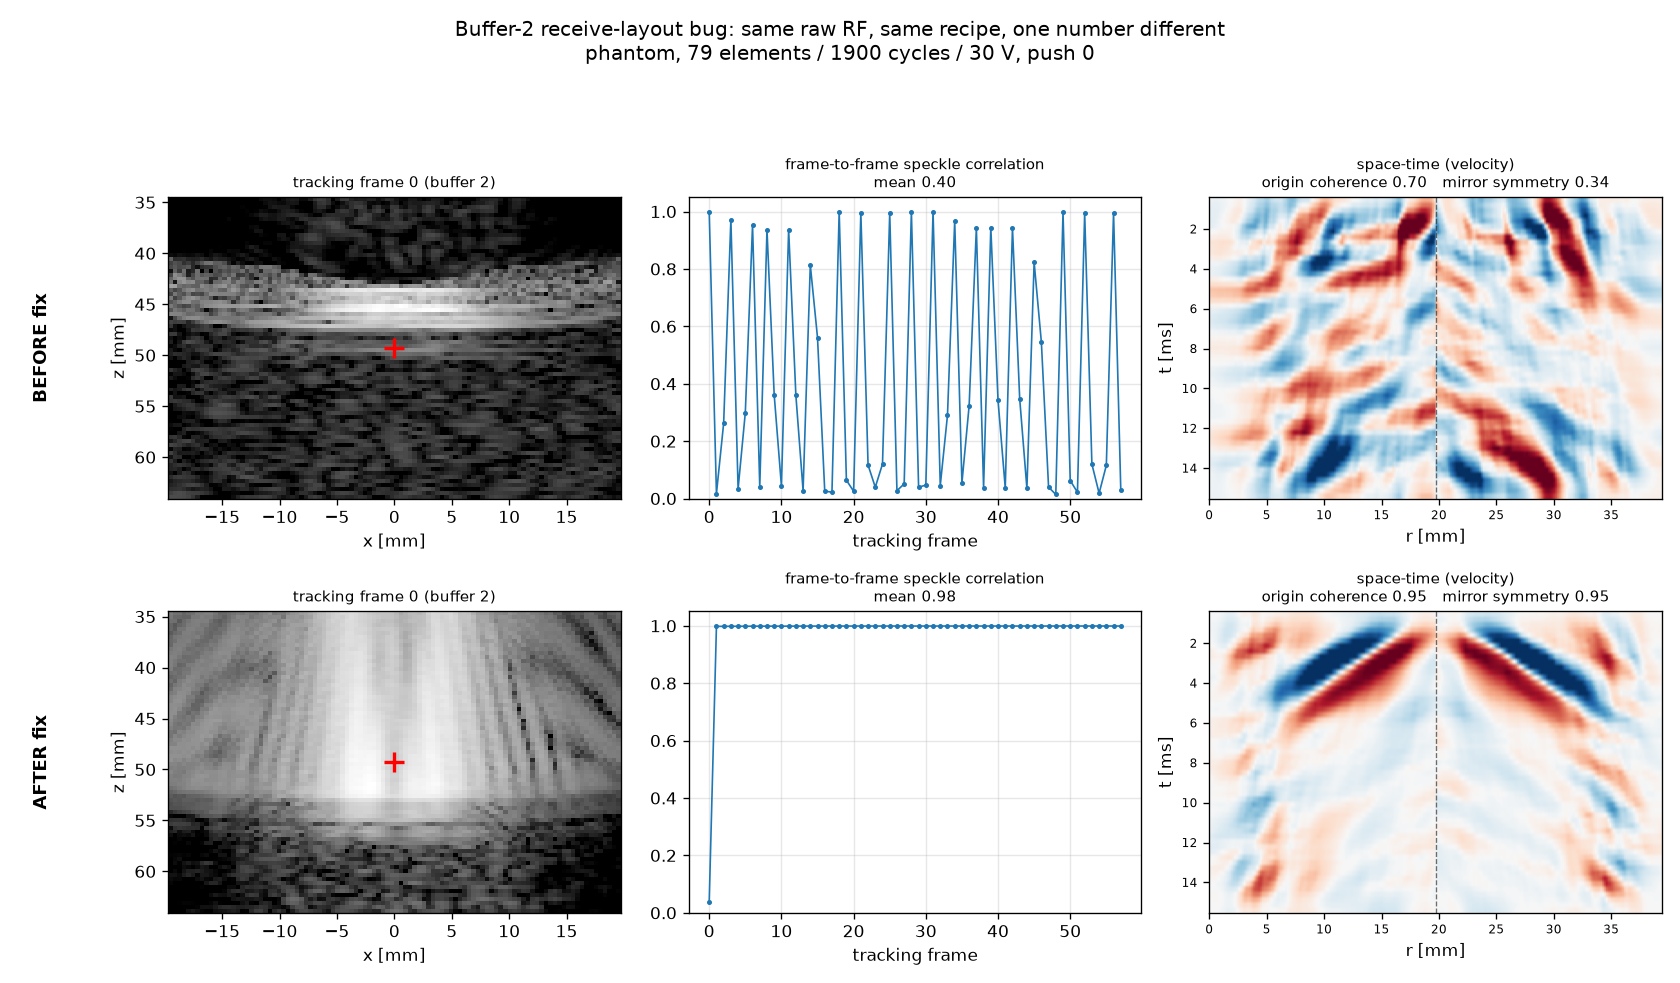
\includegraphics[width=\textwidth]{sweep_bug_before_after.png}
\caption{The receive-layout bug. Same raw RF, same processing recipe, one number different (2688 vs
3968 samples per buffer-2 acquisition). Phantom, 79 elements / 1900 cycles / 30\,V, push 0.
\textbf{Top:} the base config's layout --- the tracking frame sits at the wrong depth, the
frame-to-frame speckle correlation alternates between 1.0 and 0.02 (mean 0.40), and the space-time is
clutter (mirror symmetry 0.34). \textbf{Bottom:} the layout that matches the acquisition --- correlation
0.98, mirror symmetry 0.95.}
\label{fig:bug}
\end{figure}

% ----------------------------------------------------------------------
\subsection{Smaller problems}
% ----------------------------------------------------------------------
\begin{description}[leftmargin=1.2em,style=nextline]
  \item[Missing runtime file for the 61-element in-vivo acquisition.] The folder
  \texttt{Luuk\_61elements\_1900cycles\_25V\_...} contains only \texttt{RF\_data\_2..5.bin} --- no
  \texttt{AcquisitionParametersAndECG.mat} and no \texttt{RF\_data\_1.bin}. It was recovered from the
  session workspace dump \texttt{S5\_1\_SWI\_PulseInversion\_P46-xx\_runtime.mat} (606\,MB,
  saved \SI{10}{\minute} after that acquisition with the sequence still loaded), which carries the
  correct \texttt{SW} (61 elements, 1900 cycles, 24 frames, \texttt{WaitForRpeak}\,=\,1),
  \texttt{TPC} (profile-5 \SI{25}{\volt}), \texttt{TX} and \texttt{Receive}. Only the RF binary layout
  (\texttt{RF\_rows}/\texttt{RF\_cols}/\texttt{RF\_frames}) and \texttt{NonzeroRFcolumns} had to be
  copied from the sibling 41-element acquisition, whose buffer sizes match the file sizes byte for
  byte. New helper: \texttt{src/swp/acquisition/matlab/make\_combined\_from\_workspace.m}.
  The ECG trace for that acquisition is lost; buffer 1 (orientation B-mode) is unavailable but unused.

  \item[No hand-drawn M-lines for the new in-vivo data.] The settled workflow draws the septal M-line
  interactively per push. With 48 lines to draw and no interactive session available, they were placed
  automatically (\texttt{scripts/auto\_mline.py}): follow the bright septal ridge in a
  $\pm$\SI{9}{\milli\metre} band around the push focus, drop low-brightness columns, fit a straight
  line, and re-anchor it so it passes exactly through the push focus. A second-order fit was tried
  first and rejected --- on low-contrast frames the parabola swung off the septum. Validation against
  24 hand-drawn lines is in \S\ref{sec:q4} and Figure~\ref{fig:mline}.

  \item[No-push control window.] The control (the recipe run on pre-push frames only) is limited by
  the length of the reference block. A 50/50 split gave only 19 frames (\SI{5.1}{\milli\second}), too
  short for the slant-stack in \texttt{origin\_coherence}: the moveout ran off the end of the record
  and the normalisation broke (scores $>$\,1). An 8/31 split gives \SI{8.1}{\milli\second}, and both
  push and control are scored over \emph{that} window (the push truncated) with
  $d_\mathrm{max}$\,=\,\SI{14}{\milli\metre}, $c_\mathrm{min}$\,=\,\SI{1.5}{\metre\per\second}. The
  displayed montages still show the full \SI{16}{\milli\second} push window.

  \item[Windows \texttt{MAX\_PATH}.] The dataset paths are deep enough that
  \texttt{<folder>/AcquisitionParametersAndECG.mat} approaches the 260-character limit and the Win32
  Python layer cannot \texttt{stat} it. Everything was run through short directory junctions
  (\texttt{D:\textbackslash swp\_ph17}, \texttt{D:\textbackslash swp\_tue}, \dots), as the existing
  runbook advises.

  \item[Power-supply warning at acquisition time.] The 2026-08-17 \texttt{Readme.txt} records
  \emph{``Estimated average HV transmit supply load of 0.6\,Amps exceeds power supply capacity of
  0.5\,Amp. Actual HV transmit level may drop below the selected value.''} The profile-5
  \texttt{highVoltageLimit} was \SI{50}{\volt}, so the requested voltages were not clamped in software,
  but a rail sag under load cannot be read back from the data. \caveat{The transmit voltages in this
  log are commanded, not verified delivered.} The very clean monotonic voltage response
  (Figure~\ref{fig:scores}) argues against a large sag, but a current-probe or hydrophone check at the
  top of the sweep would settle it.
\end{description}

% ======================================================================
\section{Processing and scoring}\label{sec:methods}
% ======================================================================
Space-time plots are computed directly from the beamformed buffer-2 IQ rather than read back from the
stored \texttt{swp\_active} HDF5s, so every figure in this log is an end-to-end recomputation. Two
recipes are used, both settled in the previous report:

\begin{description}[leftmargin=1.2em,style=nextline]
  \item[Phantom recipe (\texttt{REC\_PHANTOM}, the low-SNR-robust ``id438'' family).]
  Loupas, relative-to-reference, drop frame 0 $\rightarrow$ band-pass \SIrange{80}{500}{\hertz}
  $\rightarrow$ spatial median $0.90\times\SI{2.64}{\milli\metre}$ $\rightarrow$ temporal
  moving-median 5 $\rightarrow$ 9 M-line offsets at \SI{1.09}{\milli\metre} $\rightarrow$
  outward-directional. Quantity: \emph{velocity}. M-line: horizontal at the stored push depth.
  \item[In-vivo recipe (\texttt{REC\_INVIVO}, the consensus of \texttt{configs/active.yaml}).]
  Loupas, relative-to-reference, drop frame 0 $\rightarrow$ band-pass \SIrange{120}{700}{\hertz}
  $\rightarrow$ Gaussian $\sigma_z\,0.6 \times \sigma_x\,\SI{1.2}{\milli\metre}$ $\rightarrow$
  temporal moving-mean 3 $\rightarrow$ 7 offsets at \SI{0.8}{\milli\metre} $\rightarrow$
  outward-directional. Quantity: \emph{displacement}. M-line: the septal line.
\end{description}

Two speed-free scores are reported throughout, both from the existing code base:
\textbf{origin coherence} (how well the field is a symmetric wave radiating outward from the known push
origin $r_0$ and starting near $t\approx0$; combines the two sides as a geometric mean so a one-sided
field is penalised) and \textbf{mirror symmetry} (Pearson correlation of the left- and right-lobe
envelope images as functions of distance from $r_0$ and time). Neither fits a speed, which is
deliberate: fitted speeds are unreliable at low SNR. For the phantom, both are reported as the median
[inter-quartile range] over the 10 pushes of a measurement.

\paragraph{The no-push control.} For the in-vivo data every push is additionally processed with the
\emph{same} recipe on pre-push frames only (first 8 reference frames as the reference, the remaining 31
tracked against them --- disjoint, so no data leakage). A genuine ARF wave must beat its own control.
This matters because the outward-directional filter, being anchored at $r_0$, \emph{imposes} symmetry
on non-propagating bulk motion: a symmetric ``V'' is not by itself evidence of a shear wave.

\paragraph{Acoustic output.} MI and $I_\mathrm{sppa.3}$ per cell are a linear ($\mathrm{MI}\propto V$)
and quadratic ($I_\mathrm{sppa}\propto V^2$) extrapolation of the hydrophone anchors of
\texttt{HydrophoneSafety\_Notes.md}\,\S7b: (61\,el, \SI{24.3}{\volt}, MI 1.71, $I_\mathrm{sppa.3}$ 190),
(79\,el, \SI{20.0}{\volt}, MI 1.74, 190), and the \emph{estimated} (41\,el, \SI{30}{\volt}, MI 1.52,
144). $I_\mathrm{spta.3} = I_\mathrm{sppa.3}\cdot \mathrm{PD}\cdot \mathrm{PRF_{eff}}$ with
$\mathrm{PD}=\SI{0.854}{\milli\second}$ at 1900 cycles (scaling with cycle count) and
$\mathrm{PRF_{eff}}=\SI{0.769}{\hertz}$. Limits quoted are the FDA Track-3 values: MI 1.9,
$I_\mathrm{sppa.3}$ \SI{190}{\watt\per\square\centi\metre}, $I_\mathrm{spta.3}$
\SI{720}{\milli\watt\per\square\centi\metre}. \caveat{The 41-element anchor is scaled from the 61/79
fit, not measured} --- \S\ref{sec:recommend} returns to this.

% ======================================================================
\section{Consolidated re-analysis of every hydrophone session}\label{sec:safety}
% ======================================================================
An earlier draft of this log stated that the 41-element acoustic output was scaled from the
61/79-element fit rather than measured. \bad{That was wrong.} A full 41-element voltage sweep
(15--50\,V, files \texttt{S5-1\_<V>V\_NoPreamp\_opt\_41el.hws}) was acquired on 2026-08-17 in the
same session as the preamp/no-preamp comparison, and it had simply been read from the older
narrative table (\texttt{HydrophoneSafety\_Notes.md}\,\S7b, written before that session) instead of
from the data. Every safety number in this log now comes from a single script,
\texttt{SafetyTableAll.m}, which processes \emph{both} sessions on identical conventions.

\paragraph{Method.} Depth $=|\mathrm{Pos}-\mathrm{Home}|$ from the capture notes; $f_\mathrm{awf}$
the measured $-6$\,dB fundamental (\SI{2.232}{\mega\hertz}); derating 0.3\,dB/cm/MHz; Onda
parallel-circuit sensitivity (open-circuit $M_\mathrm{oc}$ scaled by $C_h/(C_h+C_\mathrm{load})$).
With the preamp, $C_\mathrm{load}=C_\mathrm{amp}=\SI{6.1}{\pico\farad}$ and the 20\,dB gain apply;
without it, $C_\mathrm{load}$ is the cable$+$scope capacitance, calibrated from the preamp /
no-preamp ratio over the unsaturated 3--12\,V overlap $\rightarrow$
\textbf{\SI{123.3}{\pico\farad}}. $I_\mathrm{sppa.3}=\mathrm{PII.3}/\mathrm{PD}$ with PD the
$1.25\times(10\text{--}90\,\%)$ intensity-integral duration (\SI{0.852}{\milli\second} at 1900
cycles), and $I_\mathrm{spta.3}=I_\mathrm{sppa.3}\cdot\mathrm{PD}\cdot\mathrm{PRF_{eff}}$ with
$\mathrm{PRF_{eff}}=24/(1.2+30)=\SI{0.769}{\hertz}$.

\begin{table}[h]
\centering\small
\caption{\textbf{Measured} derated acoustic output of the S5-1 ARF push (session B, direct
no-preamp captures at the peak, depth \SI{3.63}{\centi\metre}). $I_\mathrm{spta.3}$ is quoted for
the 1900-cycle push. Values above an FDA limit are marked $^{\dagger}$. The 79-element row is
unreliable above 40\,V (the capture folds back --- see the text); the limit is crossed long before
that.}
\label{tab:safety}
\begin{tabular}{@{}llcccccccc@{}}
\toprule
\textbf{Elements} & \textbf{Quantity} & \textbf{15\,V} & \textbf{20\,V} & \textbf{25\,V} &
\textbf{30\,V} & \textbf{35\,V} & \textbf{40\,V} & \textbf{45\,V} & \textbf{50\,V} \\
\midrule
\multirow{3}{*}{41} & MI                & 0.71 & 0.93 & 1.15 & 1.37 & 1.64 & \textbf{1.94}$^{\dagger}$ & 2.25$^{\dagger}$ & 2.25$^{\dagger}$ \\
 & $I_\mathrm{sppa.3}$ [W/cm$^2$]        & 38 & 68 & 108 & 163 & 230$^{\dagger}$ & 291$^{\dagger}$ & 347$^{\dagger}$ & 389$^{\dagger}$ \\
 & $I_\mathrm{spta.3}$ [mW/cm$^2$]       & 25 & 45 & 71 & 107 & 151 & 191 & 228 & 256 \\
\midrule
\multirow{3}{*}{61} & MI                & 1.03 & 1.33 & 1.56 & 2.15$^{\dagger}$ & 2.66$^{\dagger}$ & 2.86$^{\dagger}$ & 3.19$^{\dagger}$ & 3.59$^{\dagger}$ \\
 & $I_\mathrm{sppa.3}$ [W/cm$^2$]        & 79 & 143 & 220$^{\dagger}$ & 327$^{\dagger}$ & 471$^{\dagger}$ & 586$^{\dagger}$ & 531$^{\dagger}$ & 690$^{\dagger}$ \\
 & $I_\mathrm{spta.3}$ [mW/cm$^2$]       & 52 & 93 & 144 & 214 & 308 & 385 & 352 & 453 \\
\midrule
\multirow{3}{*}{79} & MI                & 1.25 & 1.61 & 2.08$^{\dagger}$ & 2.65$^{\dagger}$ & 2.86$^{\dagger}$ & 2.86$^{\dagger}$ & --- & --- \\
 & $I_\mathrm{sppa.3}$ [W/cm$^2$]        & 110 & 189 & 299$^{\dagger}$ & 436$^{\dagger}$ & 481$^{\dagger}$ & 489$^{\dagger}$ & --- & --- \\
 & $I_\mathrm{spta.3}$ [mW/cm$^2$]       & 72 & 124 & 196 & 285 & 316 & 331 & --- & --- \\
\bottomrule
\end{tabular}
\end{table}

Table~\ref{tab:safety} is the measured output per aperture and voltage; Table~\ref{tab:maxv}
reduces it to the one number that drives every acquisition decision in this log.

\begin{table}[h]
\centering\small
\caption{Maximum allowed transmit voltage per aperture. \good{All three are
$I_\mathrm{sppa.3}$-limited}; MI has 20--30\,\% of headroom left at each of them. The rightmost
column is the independent session-A extrapolation, which had no 41-element data.}
\label{tab:maxv}
\begin{tabular}{@{}lcccccc@{}}
\toprule
\textbf{Elements} & \textbf{$V_\mathrm{max}$} & \textbf{binding limit} & \textbf{MI there} &
\textbf{$I_\mathrm{sppa.3}$ there} & \textbf{MI\,=\,1.9 at} & \textbf{session A $V_\mathrm{max}$} \\
\midrule
\textbf{41} & \textbf{\SI{32.0}{\volt}} & $I_\mathrm{sppa.3}$ & 1.48 & 190 & 39.3\,V & (not measured) \\
61 & \SI{23.1}{\volt} & $I_\mathrm{sppa.3}$ & 1.47 & 190 & 27.9\,V & \SI{23.6}{\volt} ($-2.4\,\%$) \\
79 & \SI{20.1}{\volt} & $I_\mathrm{sppa.3}$ & 1.62 & 190 & 23.1\,V & \SI{21.7}{\volt} ($-7.4\,\%$) \\
\bottomrule
\end{tabular}
\end{table}

\begin{figure}[t]
\centering
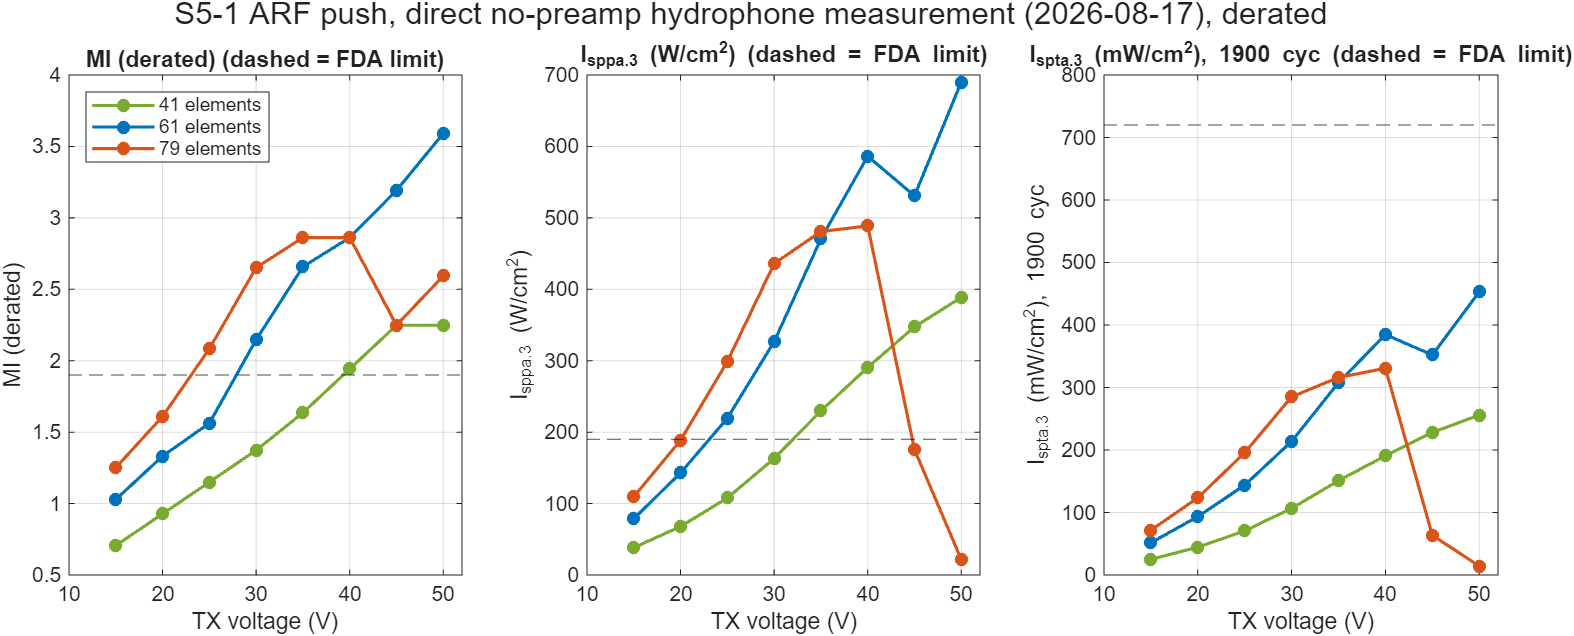
\includegraphics[width=\textwidth]{sweep_safety_measured.png}
\caption{Measured derated MI, $I_\mathrm{sppa.3}$ and $I_\mathrm{spta.3}$ of the S5-1 ARF push for
all three apertures (2026-08-17, direct no-preamp captures). Dashed lines are the FDA Track-3
limits. $I_\mathrm{sppa.3}$ is crossed first in every case; $I_\mathrm{spta.3}$ never comes close,
because the real duty cycle is 20\,Hz for 1.2\,s and then $\geq$\,30\,s off.}
\label{fig:safety}
\end{figure}

\paragraph{Cross-validation.} Session A (with preamp, 50\,$\Omega$, 2--12\,V, extrapolated) and
session B (no preamp, 1\,M$\Omega$, 15--50\,V, measured) are independent in day, electronics,
termination and transducer mounting. Where they overlap they agree to within a few per cent
(Table~\ref{tab:maxv}), which is what licenses using the session-B 41-element number on the same
footing.

\paragraph{Two 79-element datasets, and the supply-sag question.} The same folder holds a second
79-element set (\texttt{79 elements repeats\textbackslash}) with three consecutive firings stored
per capture, taken at the same nominal position. It reads a factor $\sim$1.6 \emph{lower} in
$p_r$ throughout, which would move the 79-element limit from 20\,V to beyond 50\,V --- so it
matters which one is right.
\begin{itemize}
  \item Within one repeats capture the three firings agree to 1--2\,\% (e.g. 30\,V: 50.7 / 51.4 /
  51.4\,mV). \good{There is therefore no measurable firing-to-firing transmit-supply sag}, despite
  the Verasonics 0.6\,A vs 0.5\,A warning. The 1.6$\times$ gap is \emph{between} captures.
  \item Session A --- an independent measurement --- puts the 79-element $I_\mathrm{sppa.3}=190$
  crossing at \SI{21.7}{\volt}, agreeing with the peak-optimised captures (\SI{20.1}{\volt}) and
  not with the repeats (which never reach 190 at all in 15--50\,V).
  \item The repeats were taken later without re-peaking, so they sample a slightly off-peak point.
  \caveat{The peak-optimised captures are used for the limits}, which is also the conservative
  choice.
\end{itemize}
The same question was then asked of the shear-wave data itself: across all 30 cells of the
2026-08-17 sweep, mirror symmetry as a function of push index within the 10-push burst is flat
(push 9 is $-1.5\,\%$ relative to push 0, well inside the spread; Figure~\ref{fig:pushidx}).
\good{The supply warning did not translate into a measurable output drop} in either measurement.

\begin{figure}[t]
\centering
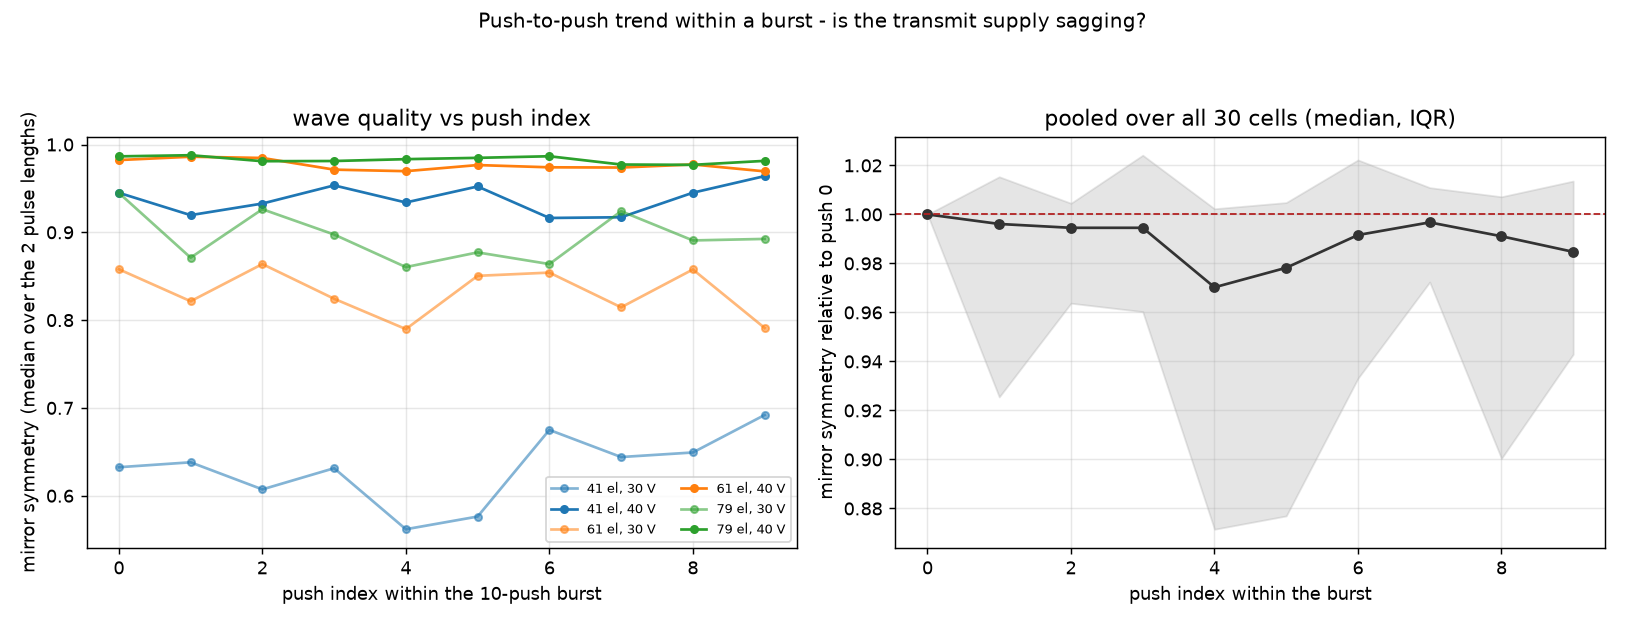
\includegraphics[width=0.92\textwidth]{sweep_push_index.png}
\caption{Shear-wave quality versus push index within the 10-push burst, 2026-08-17 sweep. Left:
per configuration. Right: pooled over all 30 cells, each normalised to its own first push. Flat ---
no transmit-supply sag within a burst.}
\label{fig:pushidx}
\end{figure}

% ======================================================================
\section{Q1 --- Reproducing the report's space-time plots}\label{sec:q1}
% ======================================================================
\good{Reproduced.} Figure~\ref{fig:q1} rebuilds the report's phantom voltage montage from the
beamformed IQ with \texttt{REC\_INVIVO}. The stored \texttt{swp\_active} HDF5s turned out to carry only
displacement views under older band tags (no velocity group, different band naming), so the montage
script could not simply re-plot them --- which is why this is a genuine end-to-end reproduction.

Both scores fall monotonically with voltage: origin coherence
$0.98 \rightarrow 0.97 \rightarrow 0.97 \rightarrow 0.95 \rightarrow 0.86 \rightarrow 0.82 \rightarrow
0.79 \rightarrow 0.75$ and mirror symmetry $0.98 \rightarrow 0.49$ from 50 to 15\,V. The report quotes
origin coherence $0.98 \rightarrow 0.69$ for the same series; the small difference at the low-voltage
end is consistent with the different colour-scale/normalisation used there and does not change the
picture. Visually the figure is the report's figure: a crisp symmetric outward wavefront at
$\geq$\,40\,V degrading smoothly into edge clutter and noise by 15\,V.

\begin{figure}[t]
\centering
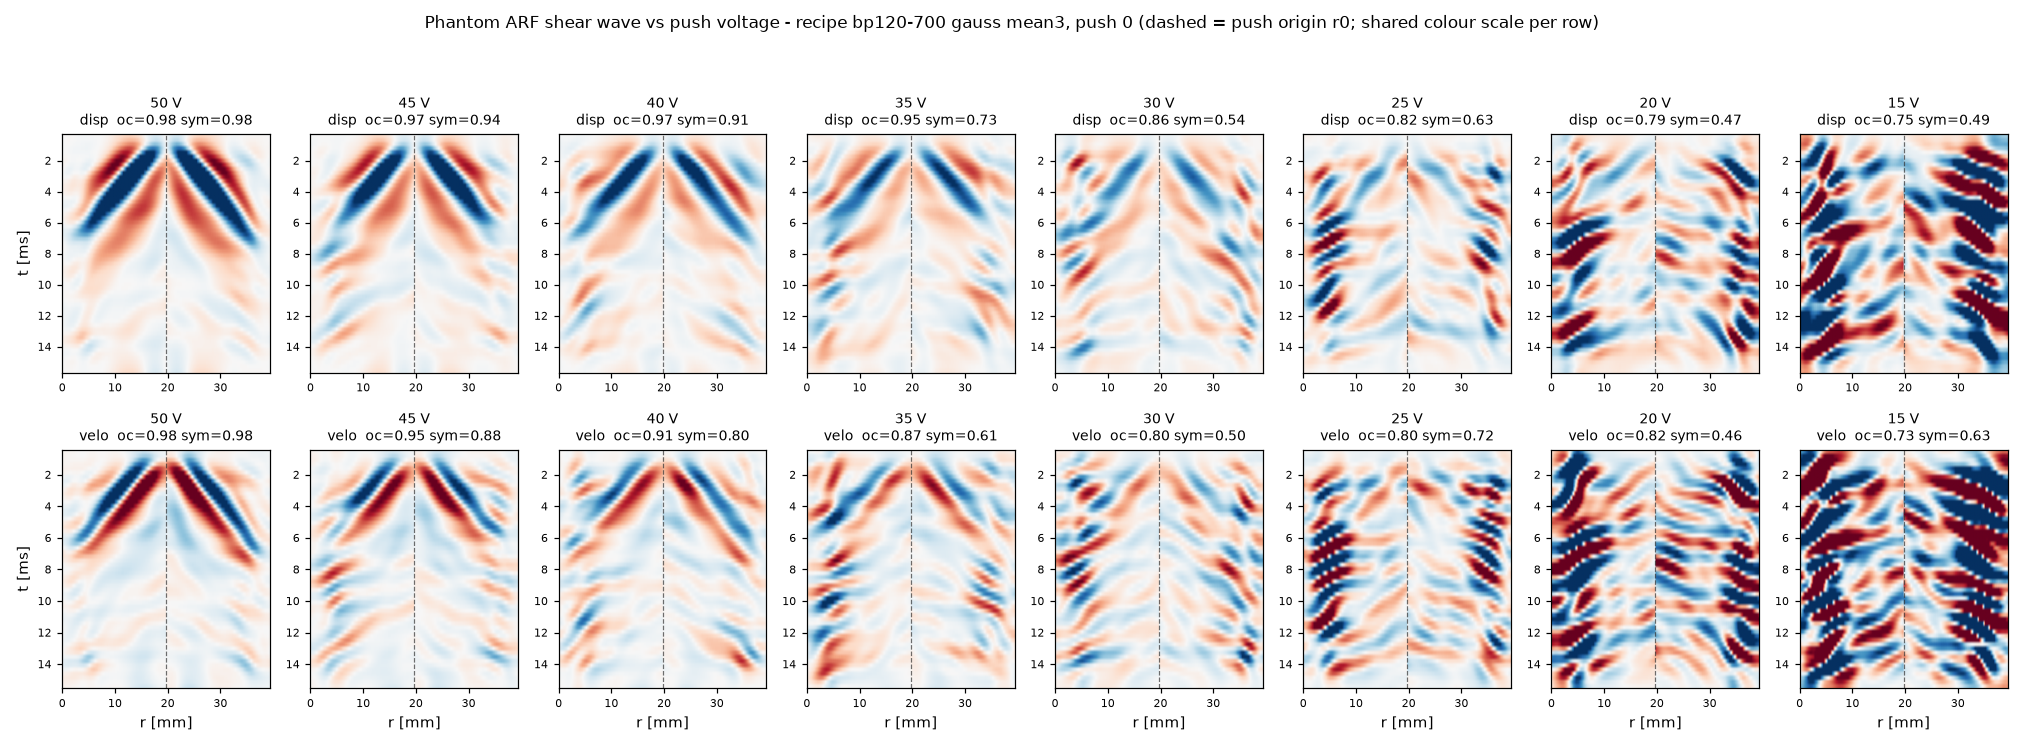
\includegraphics[width=\textwidth]{sweep_task1_voltage.png}
\caption{\textbf{Q1: reproduced.} Phantom ARF shear-wave space-time versus push transmit voltage
(50\,$\rightarrow$\,15\,V, left to right; top row displacement, bottom row velocity), recomputed from
the buffer-2 IQ with the report recipe (band-pass \SIrange{120}{700}{\hertz}, Gaussian, moving-mean 3,
7 offsets, outward-directional). Dashed line: the push origin $r_0$. Colour scale shared per row.
\texttt{oc} = origin coherence, \texttt{sym} = mirror symmetry.}
\label{fig:q1}
\end{figure}

The value of this result is that it is a positive control: the pipeline, the recipes and the scoring
all behave, so a null result on the new data (\S\ref{sec:q4}) can be attributed to the data.

% ======================================================================
\section{Q2 --- The elements $\times$ cycles $\times$ voltage sweep}\label{sec:q2}
% ======================================================================
Thirty measurements, ten pushes each, on the same phantom and with identical geometry to the reference
datasets. The two requested $5\times3$ grids are Figures~\ref{fig:grid1900} and \ref{fig:grid1500}:
rows are transmit voltage, columns are push elements, one figure per pulse length. Each panel shows the
median-symmetry push of that cell's ten; the titles carry the median [IQR] over all ten plus the
acoustic-output indices, and cells above an FDA limit are framed in red.

\begin{figure}[p]
\centering
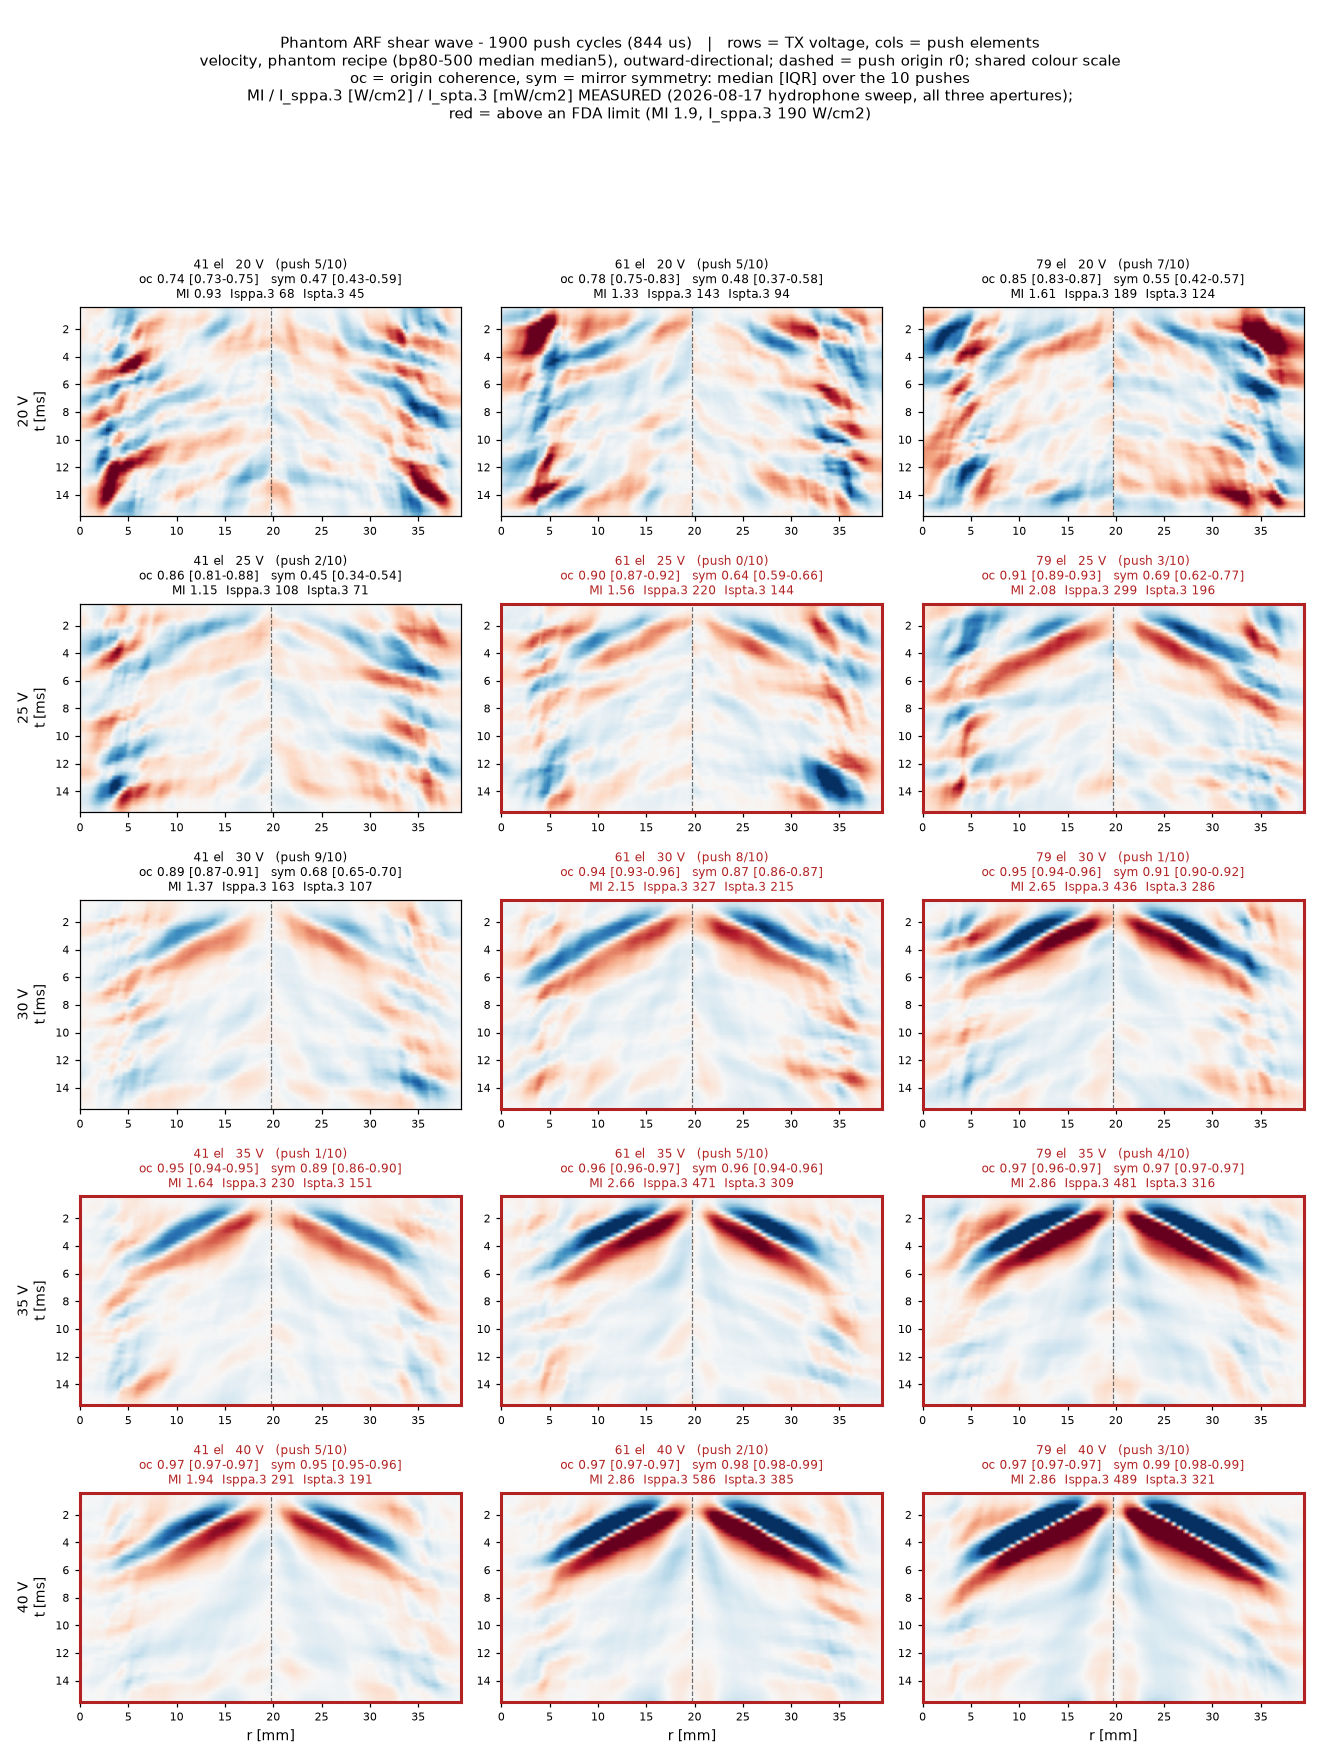
\includegraphics[width=0.86\textwidth]{sweep_grid_1900.png}
\caption{\textbf{Q2, deliverable 1 of 2: 1900 push cycles (\SI{844}{\micro\second}).} Rows: commanded
push TX voltage 20--40\,V. Columns: 41 / 61 / 79 push elements. Velocity, phantom recipe,
outward-directional; dashed line is the push origin $r_0$; shared colour scale. Red frames mark cells
above an FDA limit (MI 1.9 or $I_\mathrm{sppa.3}$ \SI{190}{\watt\per\square\centi\metre}).}
\label{fig:grid1900}
\end{figure}

\begin{figure}[p]
\centering
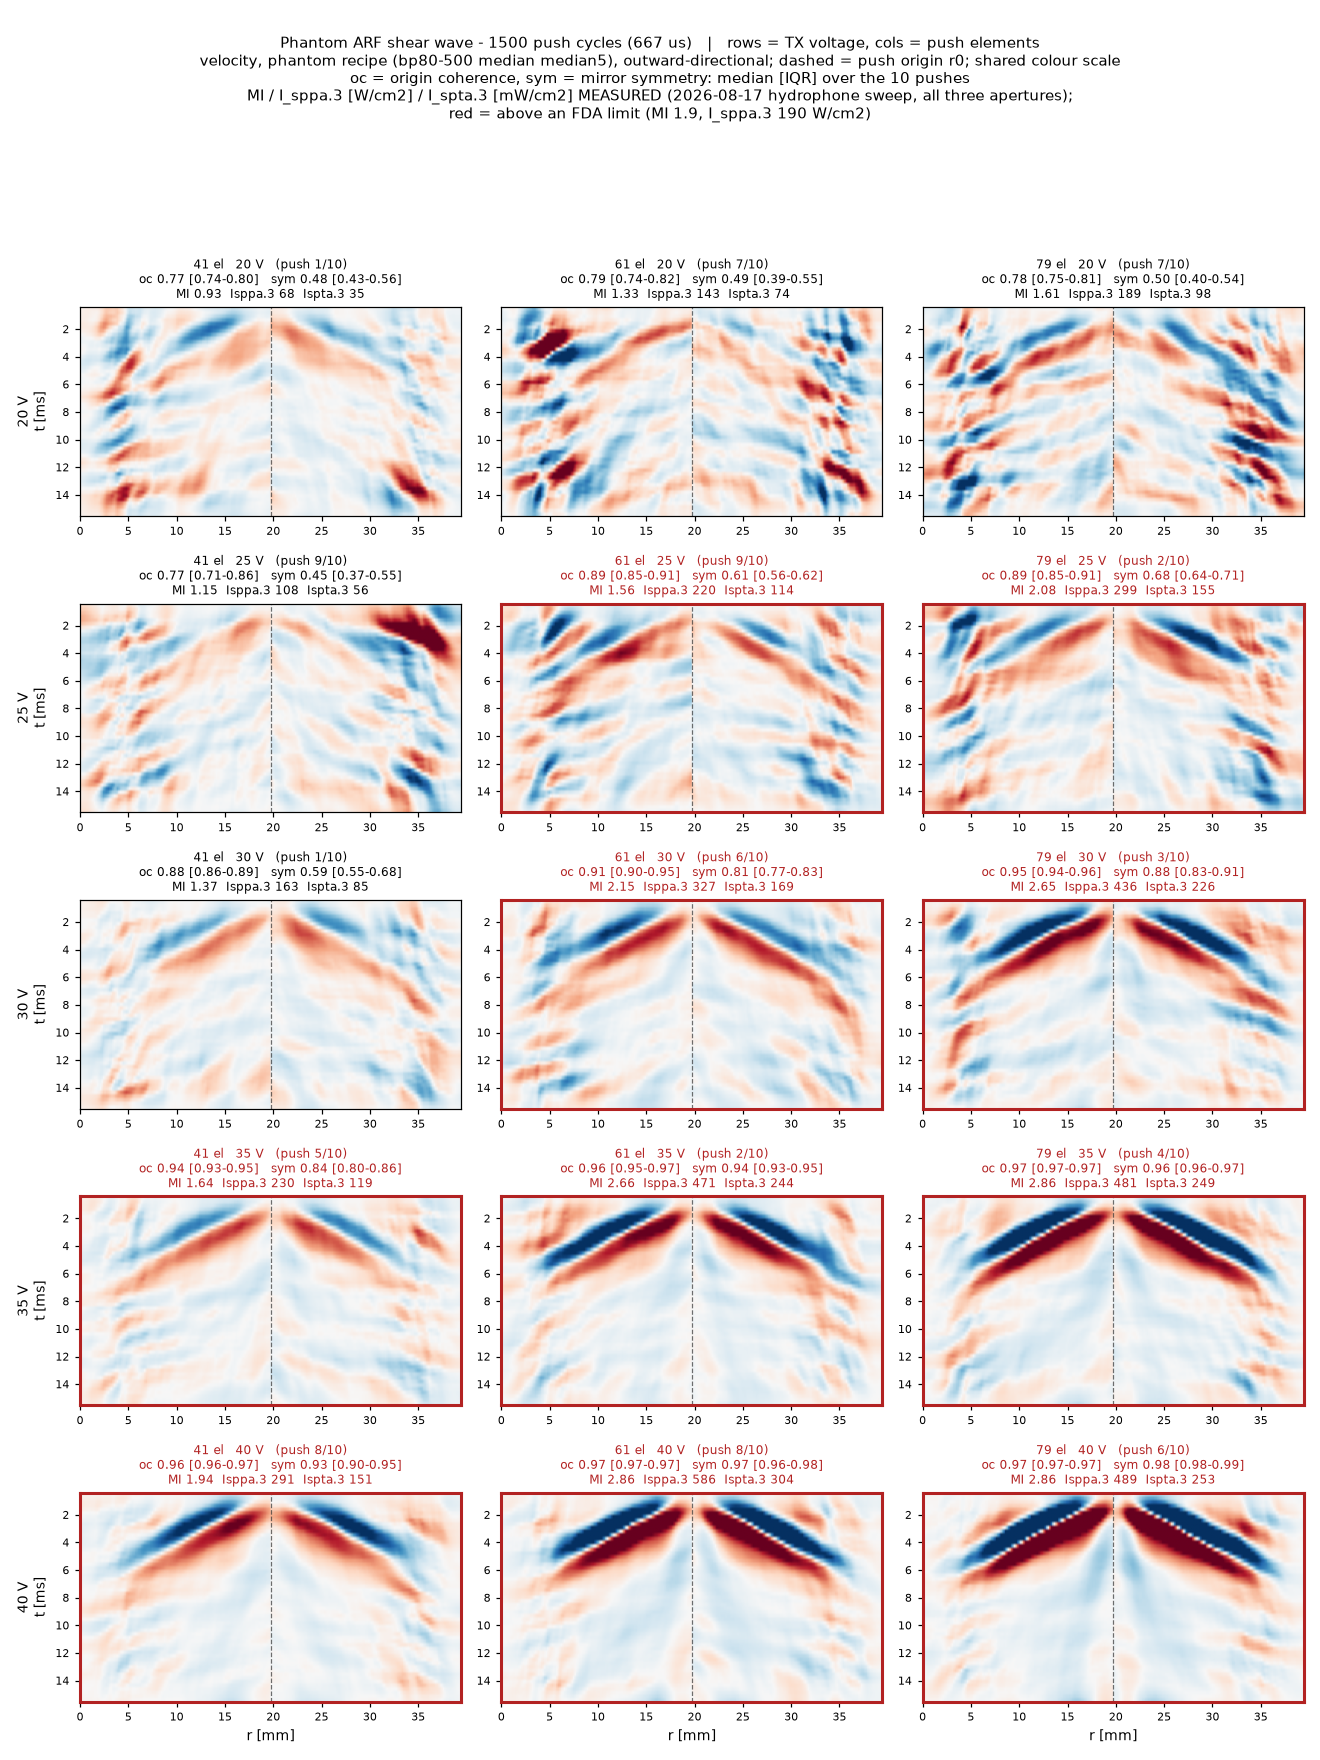
\includegraphics[width=0.86\textwidth]{sweep_grid_1500.png}
\caption{\textbf{Q2, deliverable 2 of 2: 1500 push cycles (\SI{667}{\micro\second}).} Same layout as
Figure~\ref{fig:grid1900}. Comparing the two figures cell by cell gives the pulse-length effect at
fixed aperture and voltage; it is consistently positive but small (e.g.\ 41\,el at 30\,V:
$0.59\rightarrow0.68$).}
\label{fig:grid1500}
\end{figure}

\begin{table}[t]
\centering\small
\caption{Q2 numbers: mirror symmetry (median of 10 pushes), with origin coherence in parentheses, for
all 30 cells. MI and $I_\mathrm{sppa.3}$ (\si{\watt\per\square\centi\metre}) are the extrapolated
acoustic output for that aperture/voltage; values above an FDA limit are marked $^{\dagger}$.}
\label{tab:q2}
\begin{tabular}{@{}llccccc@{}}
\toprule
\textbf{Cycles} & \textbf{Elements} & \textbf{20\,V} & \textbf{25\,V} & \textbf{30\,V} &
\textbf{35\,V} & \textbf{40\,V} \\
\midrule
\multicolumn{7}{@{}l}{\emph{MI / $I_\mathrm{sppa.3}$ (independent of pulse length)}}\\
--- & 41 & 1.01 / 64 & 1.27 / 100 & 1.52 / 144 & 1.77 / 196$^{\dagger}$ & 2.03$^{\dagger}$ / 256$^{\dagger}$ \\
--- & 61 & 1.41 / 129 & 1.76 / 201$^{\dagger}$ & 2.11$^{\dagger}$ / 290$^{\dagger}$ & 2.46$^{\dagger}$ / 394$^{\dagger}$ & 2.81$^{\dagger}$ / 515$^{\dagger}$ \\
--- & 79 & 1.74 / 190 & 2.17$^{\dagger}$ / 297$^{\dagger}$ & 2.61$^{\dagger}$ / 428$^{\dagger}$ & 3.04$^{\dagger}$ / 582$^{\dagger}$ & 3.48$^{\dagger}$ / 760$^{\dagger}$ \\
\midrule
\multirow{3}{*}{1500} & 41 & 0.48 (0.77) & 0.45 (0.77) & 0.59 (0.88) & 0.84 (0.94) & 0.93 (0.96) \\
 & 61 & 0.50 (0.79) & 0.61 (0.89) & 0.81 (0.91) & 0.94 (0.96) & 0.97 (0.97) \\
 & 79 & 0.50 (0.78) & 0.68 (0.89) & 0.89 (0.95) & 0.96 (0.97) & 0.98 (0.97) \\
\midrule
\multirow{3}{*}{1900} & 41 & 0.47 (0.74) & 0.45 (0.86) & 0.68 (0.89) & 0.89 (0.95) & 0.95 (0.97) \\
 & 61 & 0.48 (0.78) & 0.64 (0.90) & 0.87 (0.94) & 0.96 (0.96) & 0.98 (0.97) \\
 & 79 & 0.55 (0.85) & 0.69 (0.91) & 0.91 (0.95) & 0.97 (0.97) & 0.99 (0.97) \\
\bottomrule
\end{tabular}
\end{table}

\subsection{Read at matched voltage: the report replicates}
\good{H2 is confirmed as stated.} Reading Table~\ref{tab:q2} and Figure~\ref{fig:scores} along rows of
constant voltage:
\begin{itemize}
  \item Quality rises monotonically with voltage in every configuration --- the expected SNR effect,
  and a useful sanity check that the transmit voltage really did sweep despite the power-supply
  warning.
  \item At every voltage, more elements is better. At 30\,V / 1900 cycles the mirror symmetry goes
  $0.68 \rightarrow 0.87 \rightarrow 0.91$ for 41 $\rightarrow$ 61 $\rightarrow$ 79 elements.
  \item A longer pulse helps consistently but modestly (1900 vs 1500 cycles: +0.02 to +0.09 in mirror
  symmetry, largest in the mid-voltage range where the wave is marginal).
  \item Everything saturates at $\geq$\,35\,V, where all six configurations exceed 0.84.
\end{itemize}
This is the 2026-08-07 parameter sweep reproduced on independent data.

\begin{figure}[t]
\centering
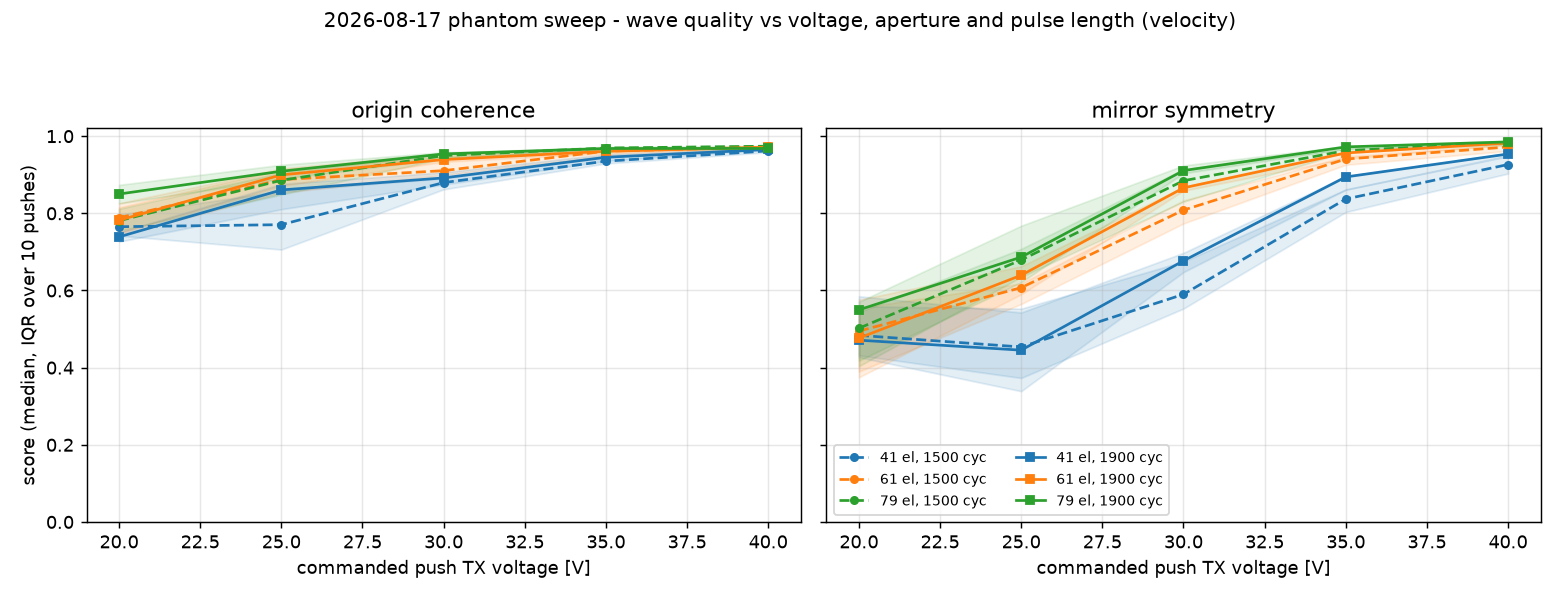
\includegraphics[width=\textwidth]{sweep_scores_voltage.png}
\caption{Q2 summary: origin coherence and mirror symmetry versus commanded transmit voltage, per
aperture (colour) and pulse length (solid = 1900 cycles, dashed = 1500). Shaded bands are the
inter-quartile range over the 10 pushes of each measurement.}
\label{fig:scores}
\end{figure}

% ----------------------------------------------------------------------
\subsection{Read at matched acoustic output: the ranking inverts}\label{sec:isosafety}
% ----------------------------------------------------------------------
The comparison above holds voltage constant. But voltage is not what we are allowed to hold constant:
$I_\mathrm{sppa.3}$ is. Because a larger aperture concentrates more energy at the focus, it reaches the
\SI{190}{\watt\per\square\centi\metre} limit at a \emph{lower} voltage
(Table~\ref{tab:maxv}) --- and the three apertures are therefore \emph{not} interchangeable at 30\,V.
Only one of the three 30\,V columns in Table~\ref{tab:q2} (41 elements) is even legal.

Re-plotting the identical 30 measurements against the \emph{measured} MI and $I_\mathrm{sppa.3}$
instead of volts (Figure~\ref{fig:iso}) inverts the ranking. Interpolating each aperture's quality
to exactly $I_\mathrm{sppa.3}=\SI{190}{\watt\per\square\centi\metre}$ --- i.e.\ each running at its
own legal maximum --- gives:

\begin{table}[h]
\centering\small
\caption{\textbf{At matched, legal acoustic output, fewer elements wins.} Each aperture is
evaluated at its own measured $V_\mathrm{max}$, where all three deliver
$I_\mathrm{sppa.3}=\SI{190}{\watt\per\square\centi\metre}$. Mirror symmetry, median of 10 pushes,
interpolated in $I_\mathrm{sppa.3}$; the three columns are independently acquired datasets.}
\label{tab:iso}
\begin{tabular}{@{}llccccc@{}}
\toprule
\textbf{Cycles} & \textbf{Configuration} & \textbf{MI there} & \textbf{$I_\mathrm{sppa.3}$} &
\textbf{08-17 TU/e} & \textbf{08-18 TU/e} & \textbf{08-18 MUMC} \\
\midrule
1900 & \textbf{41\,el @ \SI{32.0}{\volt}} & 1.48 & 190 & \textbf{0.76} & \textbf{0.77} & \textbf{0.76} \\
1900 & 61\,el @ \SI{23.1}{\volt} & 1.47 & 190 & 0.58 & 0.62 & 0.58 \\
1900 & 79\,el @ \SI{20.1}{\volt} & 1.62 & 190 & 0.55 & 0.50 & 0.55 \\
\midrule
1500 & \textbf{41\,el @ \SI{32.0}{\volt}} & 1.48 & 190 & \textbf{0.69} & \textbf{0.75} & \textbf{0.68} \\
1500 & 61\,el @ \SI{23.1}{\volt} & 1.47 & 190 & 0.56 & 0.56 & 0.52 \\
1500 & 79\,el @ \SI{20.1}{\volt} & 1.62 & 190 & 0.50 & 0.45 & 0.51 \\
\bottomrule
\end{tabular}
\end{table}

\begin{figure}[t]
\centering
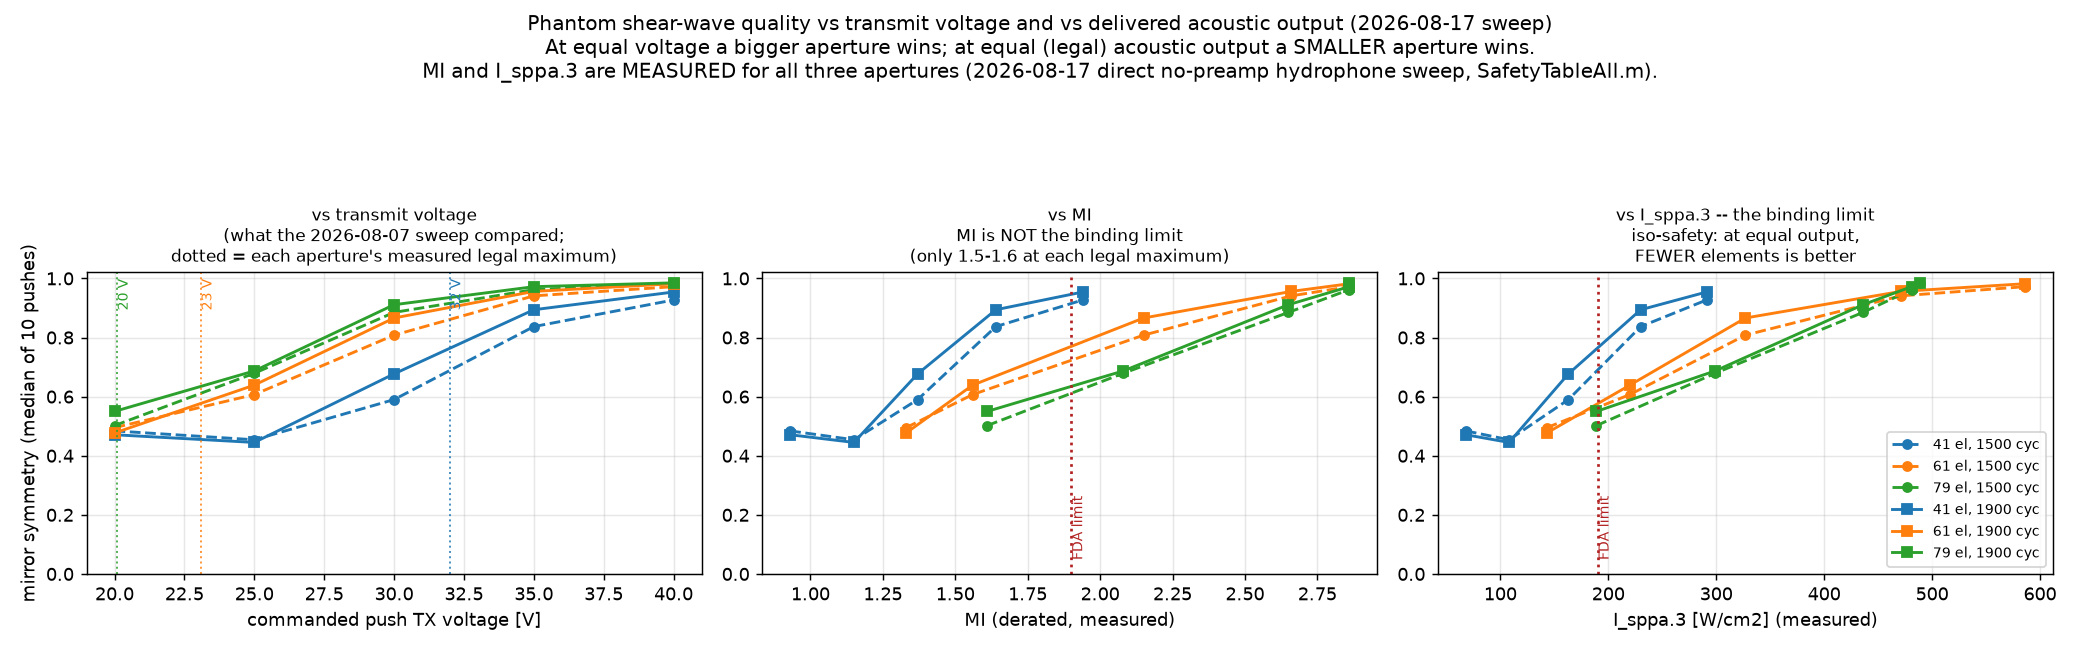
\includegraphics[width=\textwidth]{sweep_iso_safety.png}
\caption{\textbf{The same 30 measurements, three horizontal axes.} Left: versus commanded transmit
voltage --- what the 2026-08-07 sweep compared, where a bigger aperture wins; the dotted vertical
lines are each aperture's measured legal maximum. Middle: versus derated MI, which is \emph{not}
the binding limit. Right: versus $I_\mathrm{sppa.3}$, which is --- and there the 41-element curve
sits clearly \emph{above} 61 and 79. All MI / $I_\mathrm{sppa.3}$ values are measured.}
\label{fig:iso}
\end{figure}

\paragraph{Why this is physically sensible.} The radiation-force impulse delivered to the tissue scales
with the \emph{volume integral} of absorbed intensity times pulse duration, $\propto \int (2\alpha
I/c)\,\mathrm{d}V \cdot \mathrm{PD}$, whereas $I_\mathrm{sppa}$ is the \emph{peak} (spatial-peak) value.
A lower F-number raises the peak and shrinks the focal volume at the same time. Constraining the peak
therefore penalises the tighter focus: at fixed $I_\mathrm{sppa}$, the wider, longer focal region of the
smaller aperture couples more total momentum into the medium, even though its peak pressure is
identical. The measurement says this effect dominates; the more compact source that the large aperture
provides does not compensate.

\paragraph{Consequence for the previous recommendation.} The 2026-08-07 conclusion --- 61 elements ---
is correct \emph{at matched volts} and wrong \emph{at matched $I_\mathrm{sppa.3}$}. The two studies do
not disagree about any measurement; they disagree about which quantity should be held fixed. Since
2026-08-07 predates the hydrophone campaign, that constraint simply was not known at the time.

\paragraph{And no, 35\,V at 41 elements is not available.} The extrapolated table suggested a
41-element ceiling near 35\,V, which would have put the phantom quality at 0.89. The direct
measurement puts it at \SI{32.0}{\volt}: at 35\,V the measured $I_\mathrm{sppa.3}$ is
\SI{230}{\watt\per\square\centi\metre}, 21\,\% over the limit. \caveat{The realistic gain over what
was actually used in vivo is therefore from 0.68 to 0.76 in mirror symmetry, not from 0.68 to
0.89.} Useful, but not transformative.

% ----------------------------------------------------------------------
\subsection{Does the trend continue below 41 elements?}\label{sec:trend}
% ----------------------------------------------------------------------
If a smaller aperture is better at fixed output, why stop at 41? The 2026-08-07 sweep already
contains a \textbf{21-element} arm (20 and 30\,V, 1500 cycles, same phantom and geometry), so the
question can be answered without new data. Acoustic output for 21 elements is not measured; it is
scaled using the \emph{measured} focal-gain exponent, obtained by fitting $p_r\propto N^q$ to the
41/61/79-element MI at an unsaturated 20\,V:
\begin{equation}
q = 0.842 \quad\Longrightarrow\quad I_\mathrm{sppa}\propto N^{1.68}.
\end{equation}

Two constraints then bound the aperture from opposite sides:
\begin{itemize}
  \item \textbf{from above} --- $I_\mathrm{sppa.3}\leq\SI{190}{\watt\per\square\centi\metre}$ forces
  the voltage down as $N$ grows (32 / 23 / 20\,V at 41 / 61 / 79 elements);
  \item \textbf{from below} --- the transmit hardware stops at 50\,V, so a small enough aperture can
  no longer reach the limit at all. The crossover is at
  $N = 41\,(190/389)^{1/1.68} \approx \textbf{27 elements}$: below that, the safety limit stops
  binding and the \emph{hardware} does.
\end{itemize}

\good{So there is an optimum, and 21 elements is past it.} At 21 elements the full 50\,V delivers
only $I_\mathrm{sppa.3}\approx\SI{126}{\watt\per\square\centi\metre}$ --- two-thirds of the legal
ceiling, unreachable. The measured quality behaves accordingly: 21 elements scores 0.47 at 20\,V and
0.48 at 30\,V, i.e.\ \bad{flat}, sitting on the noise floor and barely responding to voltage, while
41 elements goes 0.52 $\rightarrow$ 0.64 over the same range. This is exactly the
``insufficient acoustic power to cause meaningful displacement'' regime.

\begin{figure}[t]
\centering
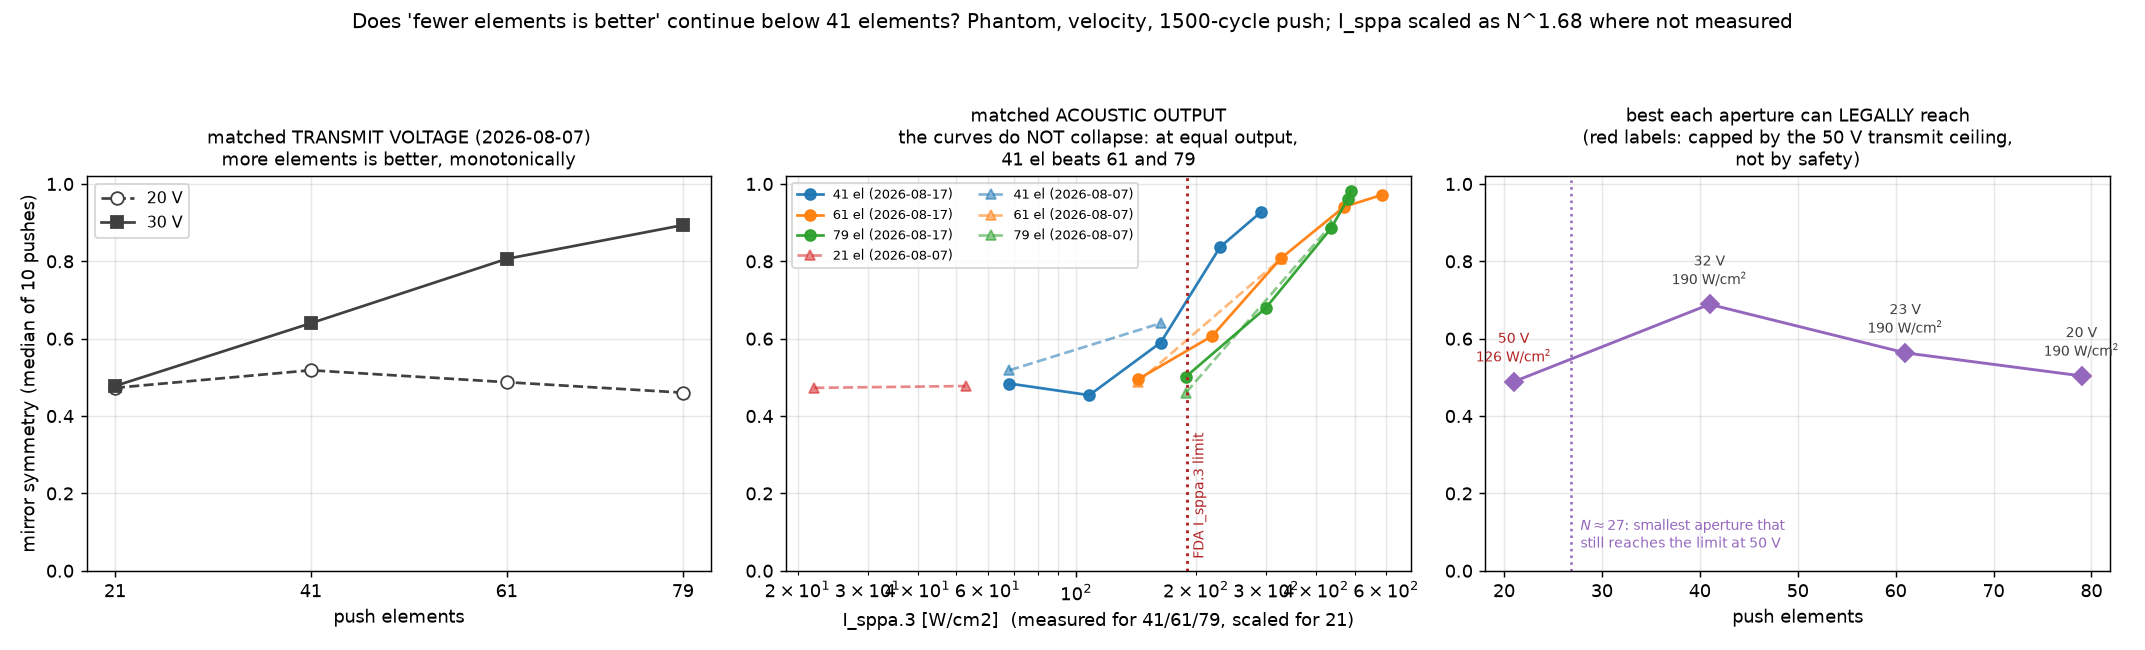
\includegraphics[width=\textwidth]{sweep_aperture_trend.png}
\caption{Extending the aperture trend down to 21 elements. \emph{Left:} at matched transmit voltage
(2026-08-07) the ordering is monotone in $N$ at 30\,V; at 20\,V every aperture is at the noise floor
and the ordering carries no information. \emph{Middle:} the same points plus the 2026-08-17 sweep
against acoustic output --- the curves do \emph{not} collapse onto one, so aperture matters
independently of output. \emph{Right:} the best each aperture can legally reach. The curve peaks at
41 elements: 21 elements is capped by the 50\,V transmit ceiling at only 126\,W/cm$^2$, 61 and 79
are capped by safety at a voltage too low to be useful.}
\label{fig:trend}
\end{figure}

\paragraph{What is untested.} The interval \textbf{27--41 elements} has no quality data at all. The
argument above predicts that 31 elements at $\approx$\,\SI{41}{\volt}, or 27 elements at
$\approx$\,\SI{50}{\volt} --- both reaching the full \SI{190}{\watt\per\square\centi\metre} with a
larger focal volume than 41 elements --- should beat 41\,el\,@\,\SI{32}{\volt}. That is a cheap
phantom experiment and it is the one worth doing next (\S\ref{sec:next}). It is a prediction from an
extrapolated output scaling, so it may not survive contact with the data: the 41-element peak in
Figure~\ref{fig:trend} (right) may simply be the optimum.

% ======================================================================
\section{Q3 --- TU/e versus MUMC S5-1}\label{sec:q3}
% ======================================================================
\good{H3 is rejected: the two probes are indistinguishable.} Both swept the full
$3\times2\times5$ grid on the same phantom within \SI{45}{\minute}, 10 pushes per cell, plus one
focused B-mode of a resolution phantom each.

Pooling all 30 cells (Figure~\ref{fig:probe}):
\begin{itemize}
  \item \textbf{MUMC $-$ TU/e} (same day, same phantom): mean $-0.004$, median $-0.011$, RMS $0.039$,
  worst single cell $0.087$ in mirror symmetry.
  \item \textbf{2026-08-18 TU/e $-$ 2026-08-17 TU/e} (the \emph{same} probe, one day apart, re-coupled):
  mean $+0.002$, median $+0.005$, RMS $0.034$, worst cell $0.086$.
\end{itemize}
The probe-to-probe difference is the same size as the day-to-day repeatability of a single probe, i.e.
it is measurement noise. The resolution-phantom B-modes (Figure~\ref{fig:bmode}) agree as well; the
apparent depth difference is a lateral placement difference of the wire column, not sensitivity.

Two things follow. First, \textbf{the transducer is not what limits the in-vivo measurement} --- a real
possibility worth eliminating, and now eliminated. Second, this dataset doubles as an
\emph{independent replication} of Q2: both probes reproduce the iso-output ranking of
Table~\ref{tab:iso} to within 0.05.

\begin{figure}[t]
\centering
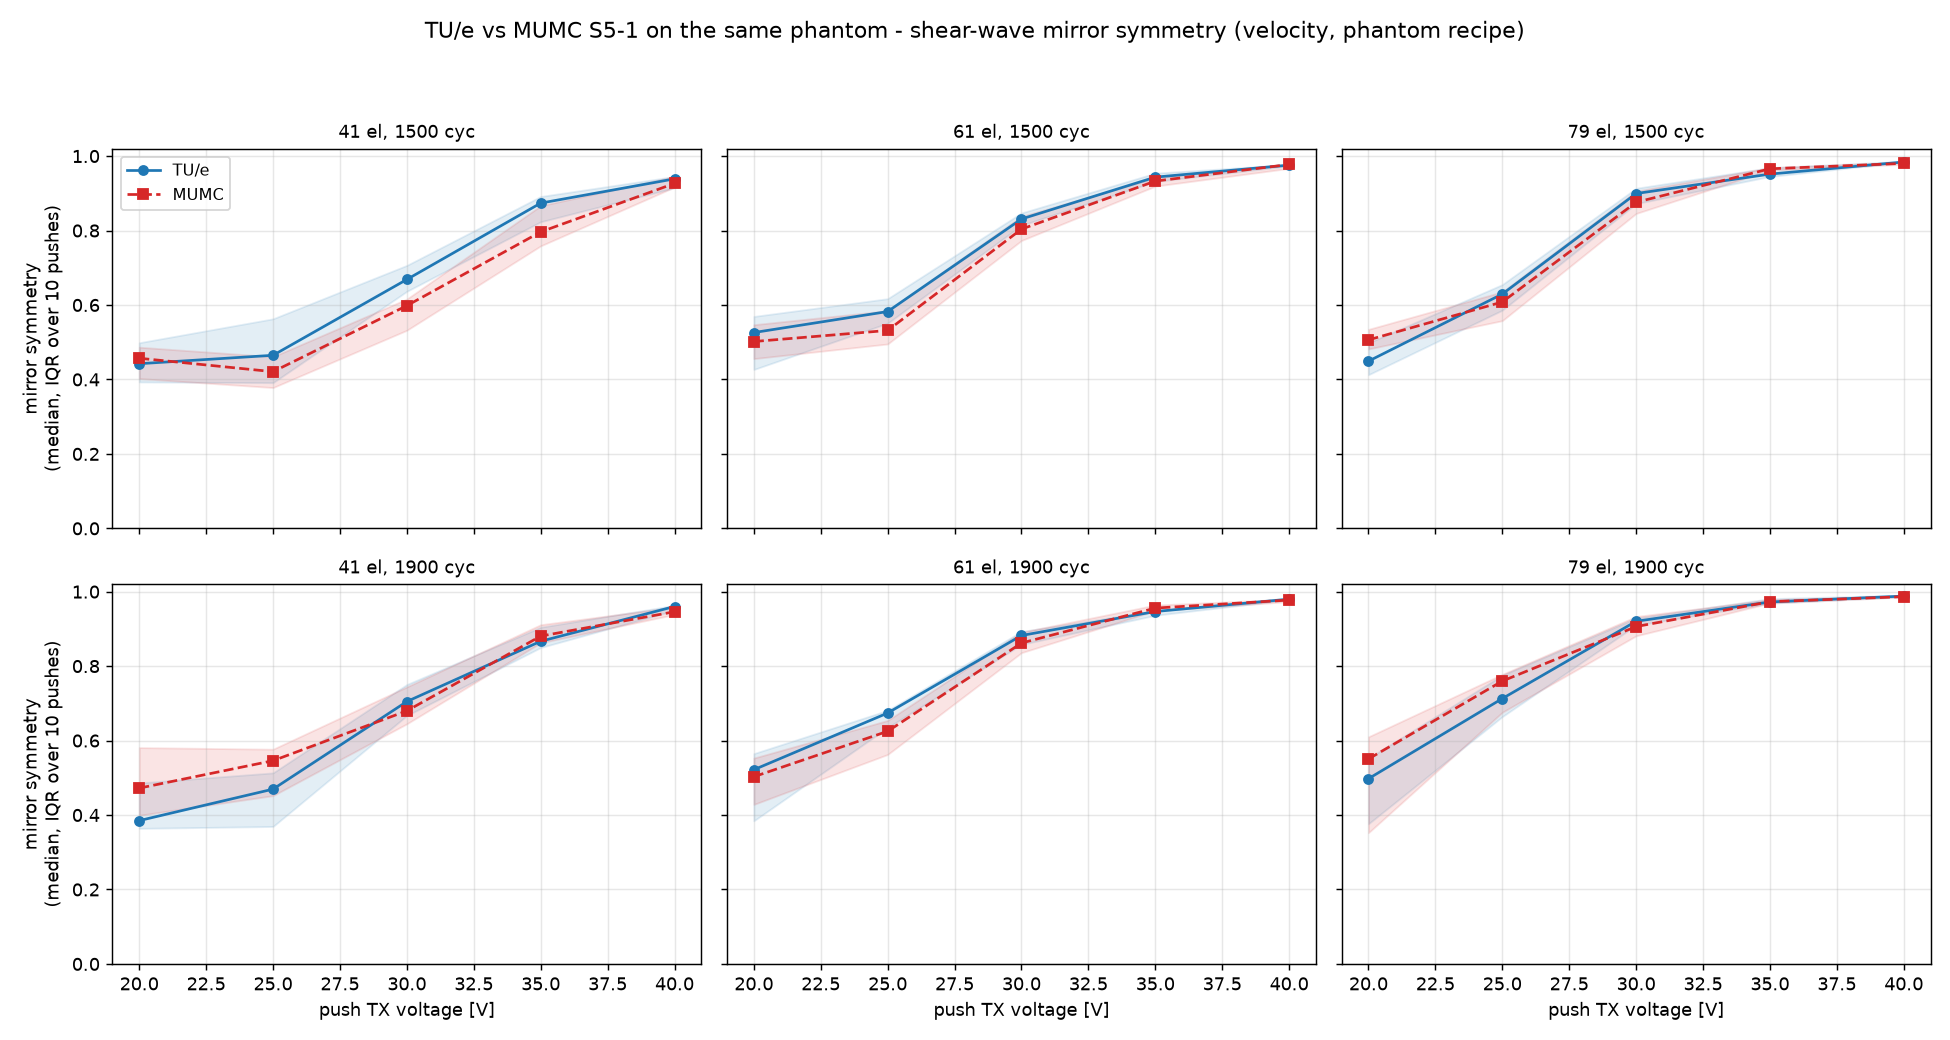
\includegraphics[width=\textwidth]{sweep_probe_summary.png}
\caption{Q3: mirror symmetry versus transmit voltage for the TU/e (blue, solid) and MUMC (red, dashed)
S5-1, one panel per aperture and pulse length, on the same phantom. Shaded bands are the IQR over 10
pushes. The curves overlap within the IQR essentially everywhere.}
\label{fig:probe}
\end{figure}

\begin{figure}[t]
\centering
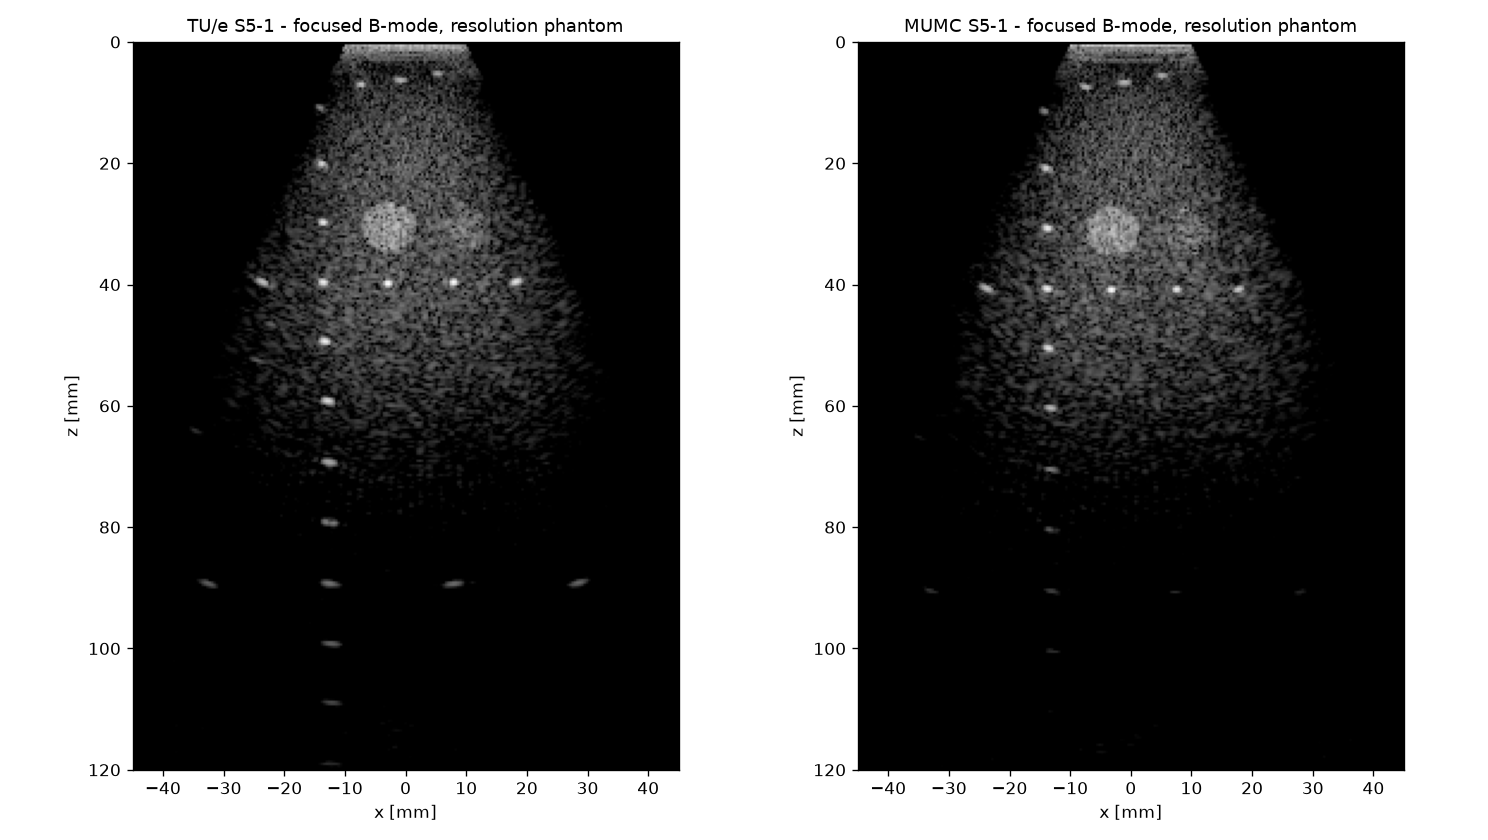
\includegraphics[width=0.86\textwidth]{sweep_probe_bmode.png}
\caption{Q3: focused B-mode of the resolution phantom, both probes, same dynamic range. Comparable
wire-target resolution and penetration.}
\label{fig:bmode}
\end{figure}

% ======================================================================
\section{Q4 --- In vivo: does the changed push help?}\label{sec:q4}
% ======================================================================
\bad{H4 is rejected: neither configuration beats its own no-push control.}

Two acquisitions on the same subject, minutes apart, both R-peak triggered
(\texttt{SW.WaitForRpeak}\,=\,1 --- a change from the free-running 2026-08-04 data, and a genuine
improvement in its own right), 24 pushes at \SI{20}{\hertz}. Push $k$ therefore falls at
$\approx 50k$\,ms after the R-peak in \emph{both}, so the two are comparable push by push in cardiac
phase --- something the older data could not support.

\paragraph{M-line validation.} Before trusting the automatic septal M-lines, they were checked against
the 24 hand-drawn lines of the 2026-08-04 40\,V acquisition (Figure~\ref{fig:mline}): mean
auto-minus-manual origin coherence $-0.014$, mirror symmetry $+0.058$, mean line separation
\SI{2.4}{\milli\metre}. \good{No systematic bias}, but \caveat{the per-push scatter is large} --- which
is consistent with the M-line-variance section of the previous report. The automatic lines are
adequate for a conclusion pooled over 24 pushes; they are not adequate for reading a single push
quantitatively.

\begin{figure}[t]
\centering
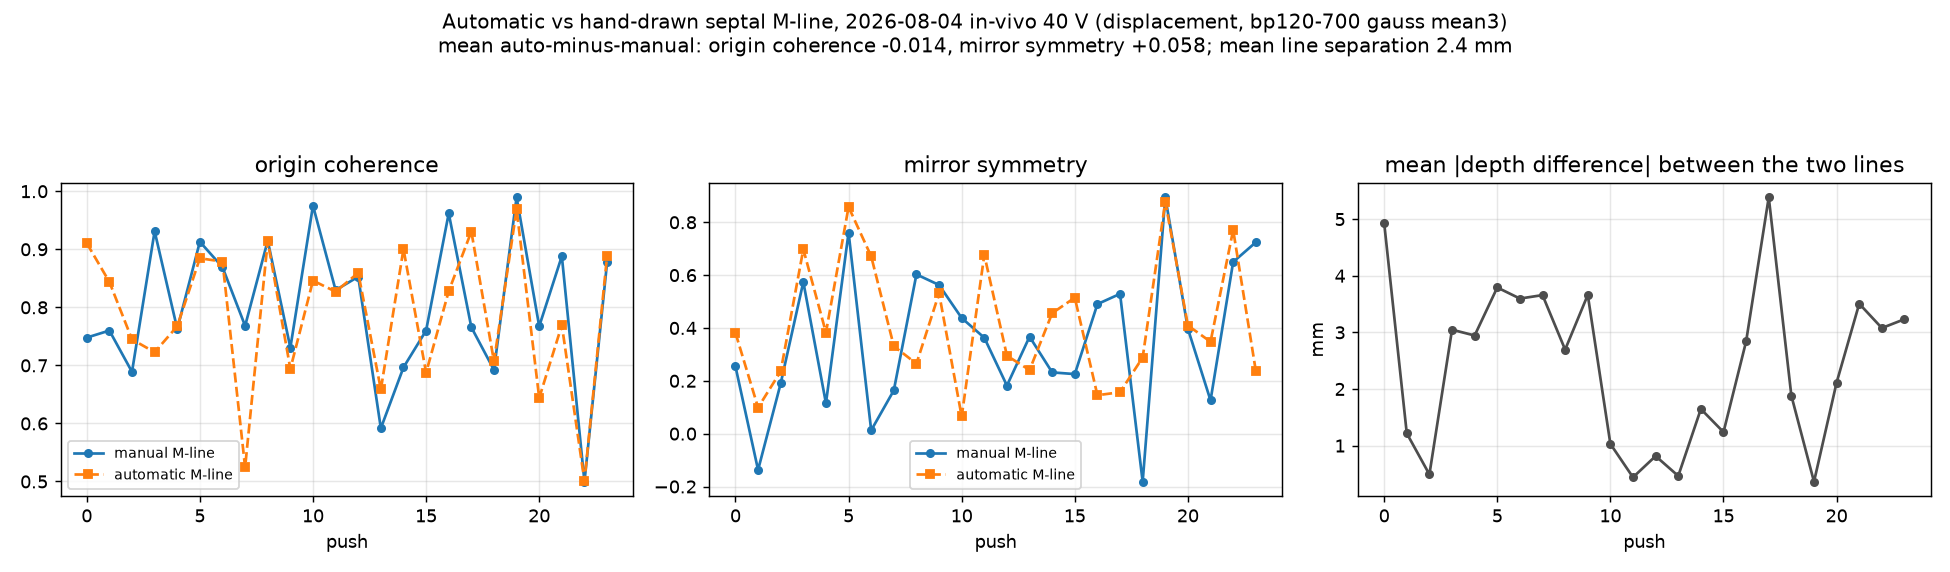
\includegraphics[width=\textwidth]{sweep_mline_validation.png}
\caption{Automatic versus hand-drawn septal M-line on the 2026-08-04 in-vivo 40\,V acquisition, per
push. Left/middle: the two scores track each other with no systematic offset. Right: mean depth
separation between the two curves.}
\label{fig:mline}
\end{figure}

\paragraph{Result.} Figure~\ref{fig:ivsum} plots both configurations against cardiac phase, together
with their controls. The push-minus-control contrast oscillates about zero for both; there is no
systematic positive offset at any phase. Table~\ref{tab:invivo} pools the 24 pushes of each
acquisition and adds the two older free-running acquisitions for reference.

\begin{table}[h]
\centering\small
\caption{Q4: pooled push-minus-control origin coherence. A configuration that images a real ARF wave
should be clearly positive. None is. MI/$I_\mathrm{sppa.3}$ marked $^{\dagger}$ exceed an FDA limit.}
\label{tab:invivo}
\begin{tabular}{@{}llccrr@{}}
\toprule
\textbf{Acquisition} & \textbf{Gating} & \textbf{MI} & \textbf{$I_\mathrm{sppa.3}$} &
\textbf{median $\Delta$OC} & \textbf{fraction $>0$} \\
\midrule
2026-08-04 \quad 41\,el / 1500\,cyc / 40\,V & free-running & \textbf{1.94}$^{\dagger}$ & 291$^{\dagger}$ & $+0.017$ & 0.58 \\
2026-08-04 \quad 41\,el / 1500\,cyc / 30\,V & free-running & 1.37 & 163 & $-0.005$ & 0.46 \\
2026-08-18 \quad 41\,el / 1500\,cyc / 30\,V & R-peak & 1.37 & 163 & $-0.052$ & 0.42 \\
2026-08-18 \quad 61\,el / 1900\,cyc / 25\,V & R-peak & 1.56 & 220$^{\dagger}$ & $-0.043$ & 0.33 \\
\bottomrule
\end{tabular}
\end{table}

\begin{figure}[t]
\centering
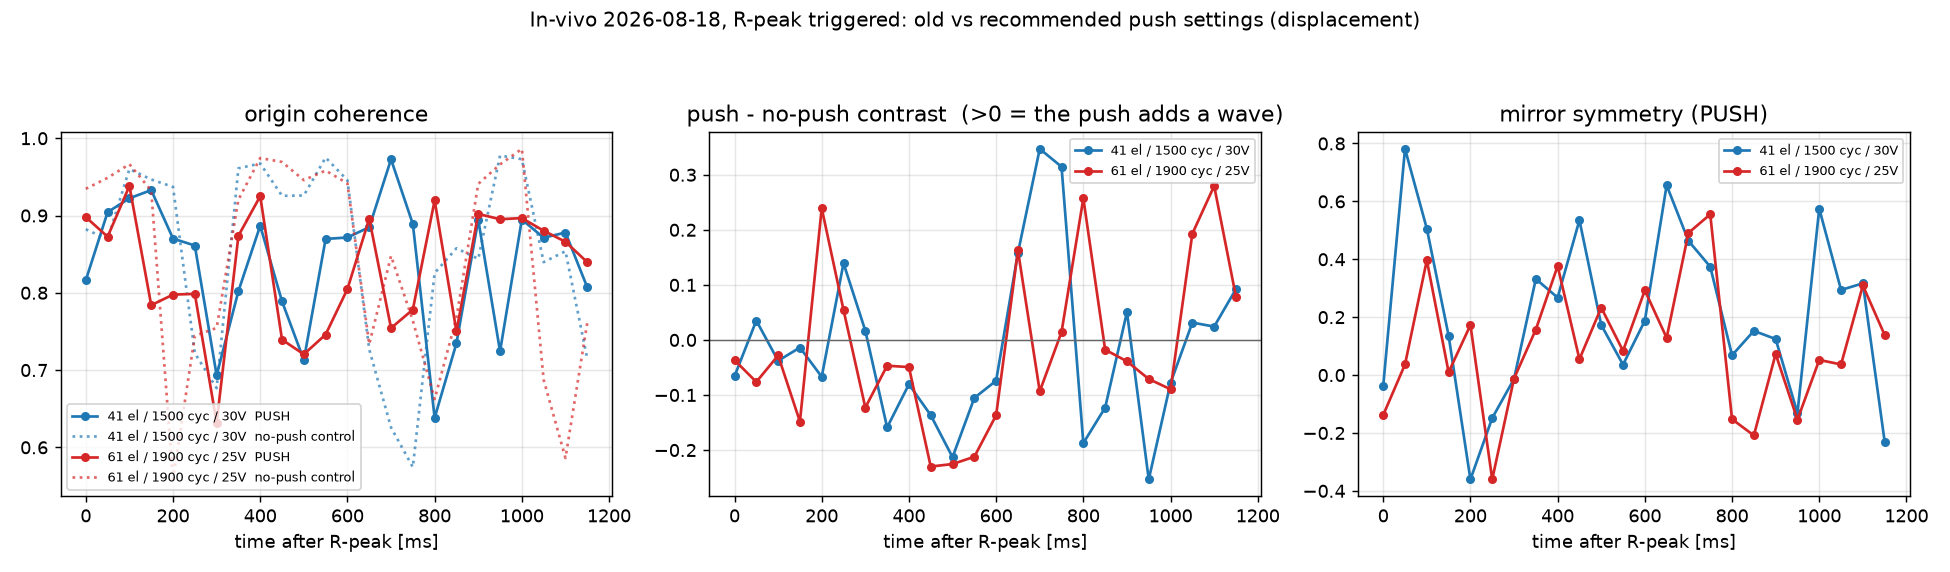
\includegraphics[width=\textwidth]{sweep_invivo_summary.png}
\caption{Q4: in-vivo scores versus time after the R-peak. Left: origin coherence for the push (solid)
and its own no-push control (dotted) --- note how closely the control tracks the push. Middle: the
contrast, which is what matters; it swings either side of zero with cardiac phase and has no
systematic positive offset. Right: mirror symmetry of the push.}
\label{fig:ivsum}
\end{figure}

\begin{figure}[p]
\centering
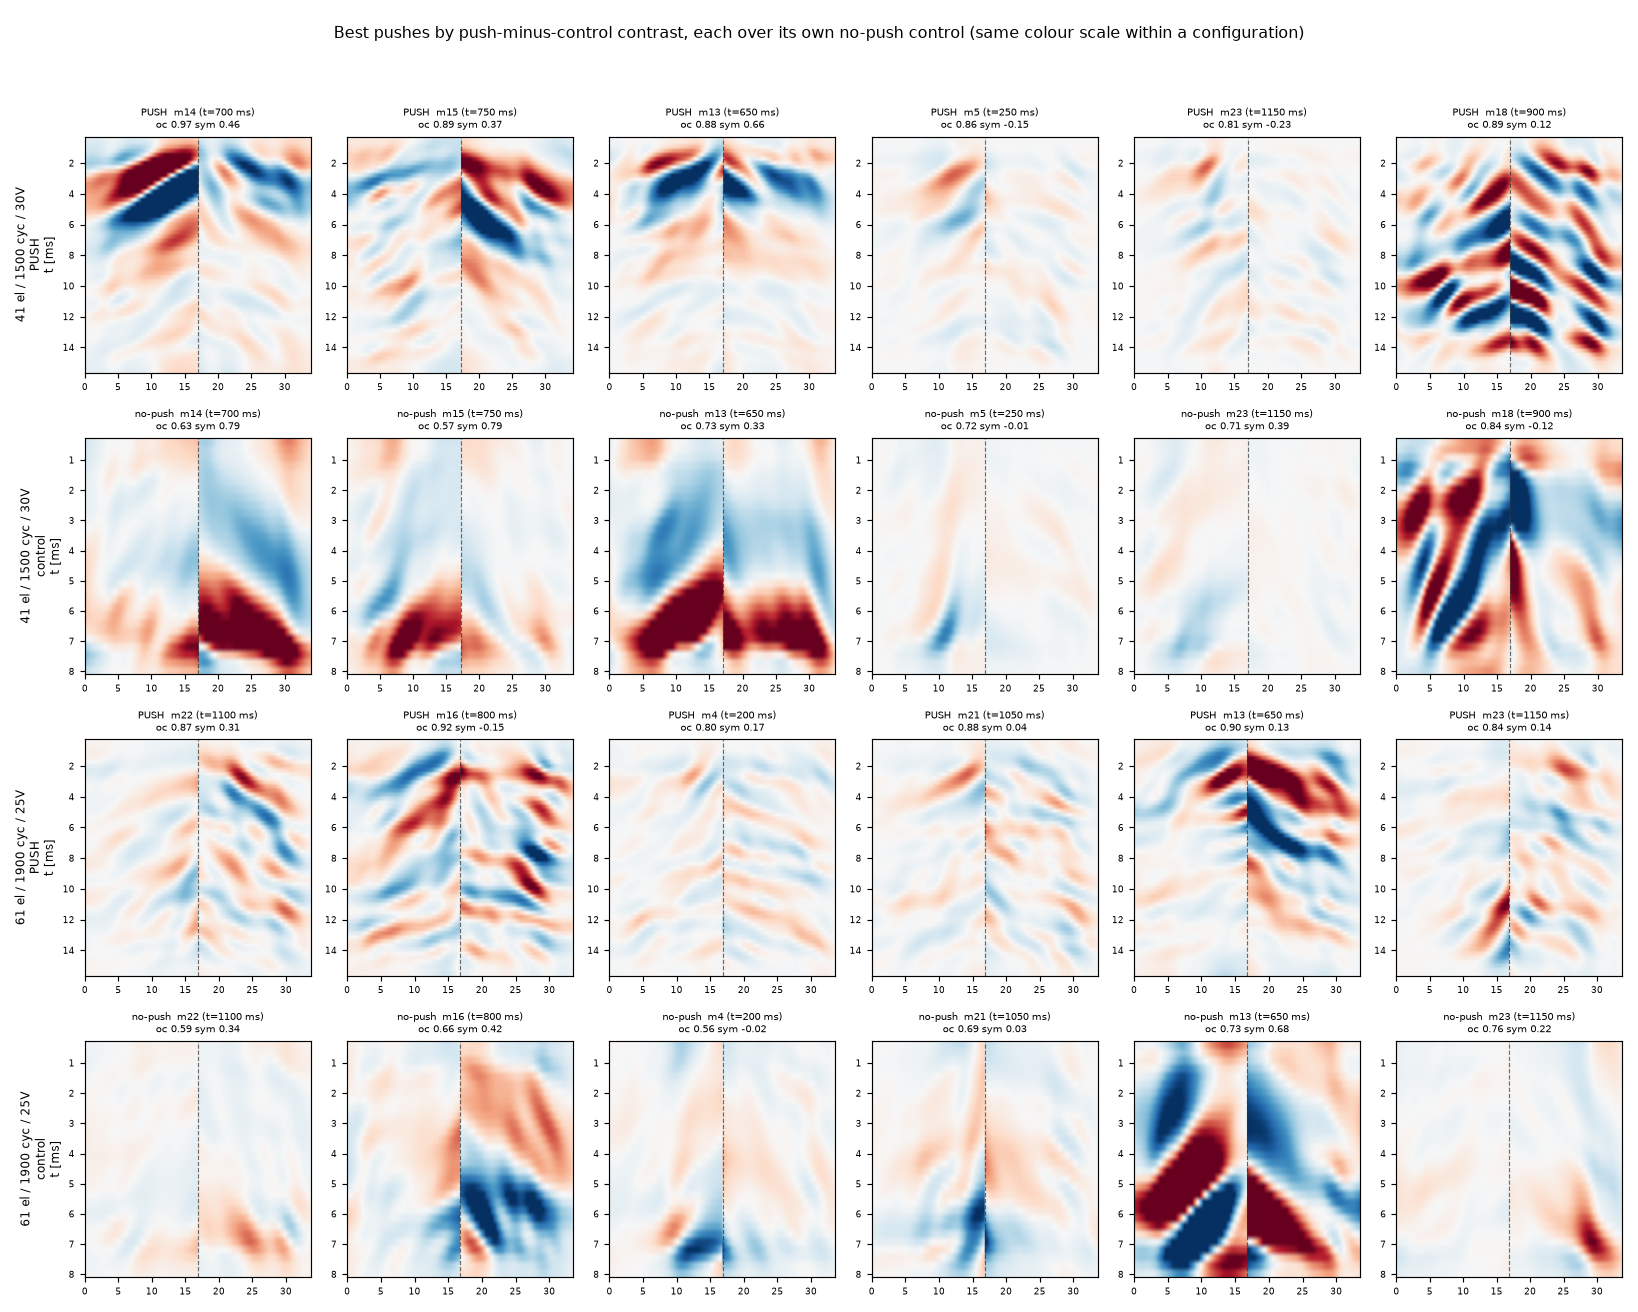
\includegraphics[width=0.95\textwidth]{sweep_invivo_best.png}
\caption{Q4: the six pushes of each configuration with the highest push-minus-control contrast, each
shown above its own no-push control on a common colour scale. A few quiet-phase pushes of the
41-element acquisition (m13--m15, 650--\SI{750}{\milli\second} after the R-peak) do show a fan opening
from $r_0$ early in the record, but their controls carry comparable energy, and none is the clean
symmetric V that the phantom produces with the same recipe.}
\label{fig:ivbest}
\end{figure}

\begin{figure}[t]
\centering
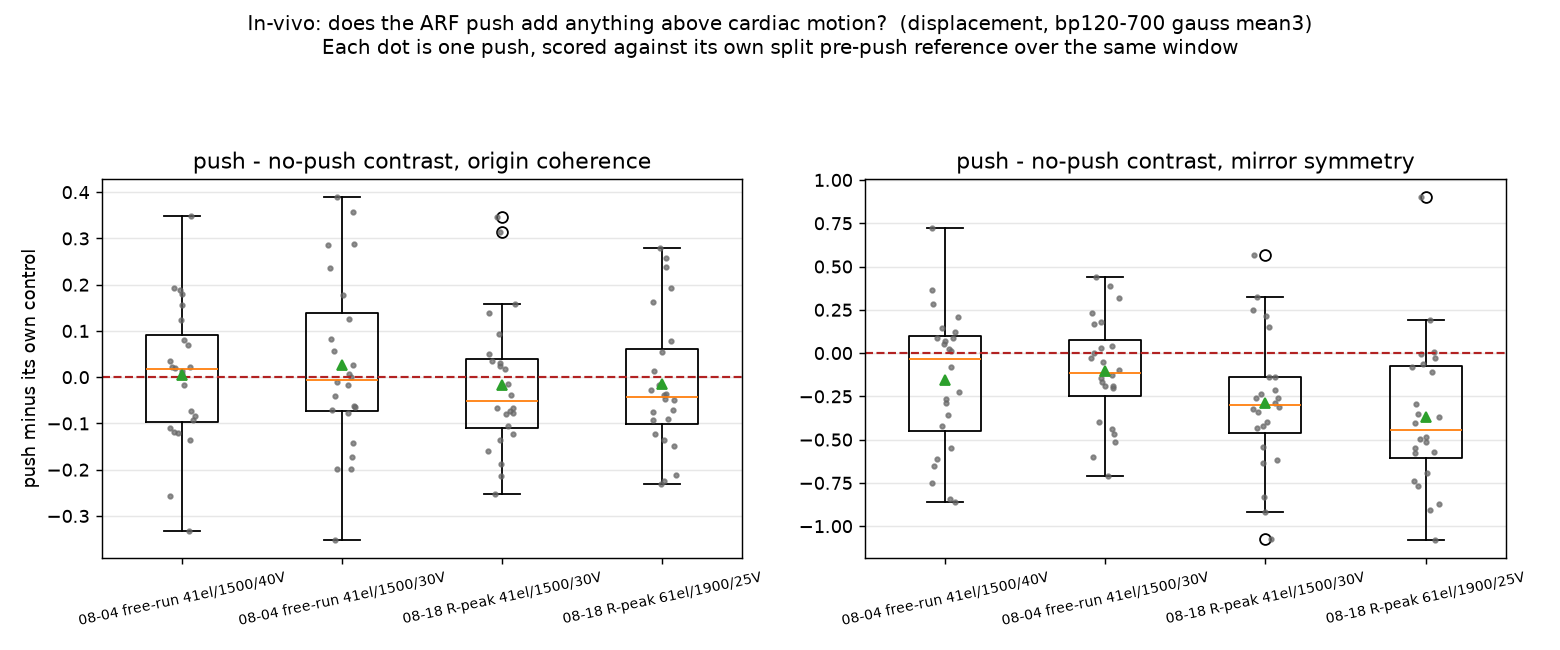
\includegraphics[width=0.9\textwidth]{sweep_invivo_contrast.png}
\caption{Q4: push-minus-control contrast pooled per configuration; every dot is one push. All four
acquisitions sit on zero. The 61-element acquisition is, if anything, marginally worse than the old
41-element one --- which is what the iso-output result of \S\ref{sec:isosafety} predicts.}
\label{fig:ivcontrast}
\end{figure}

\begin{figure}[p]
\centering
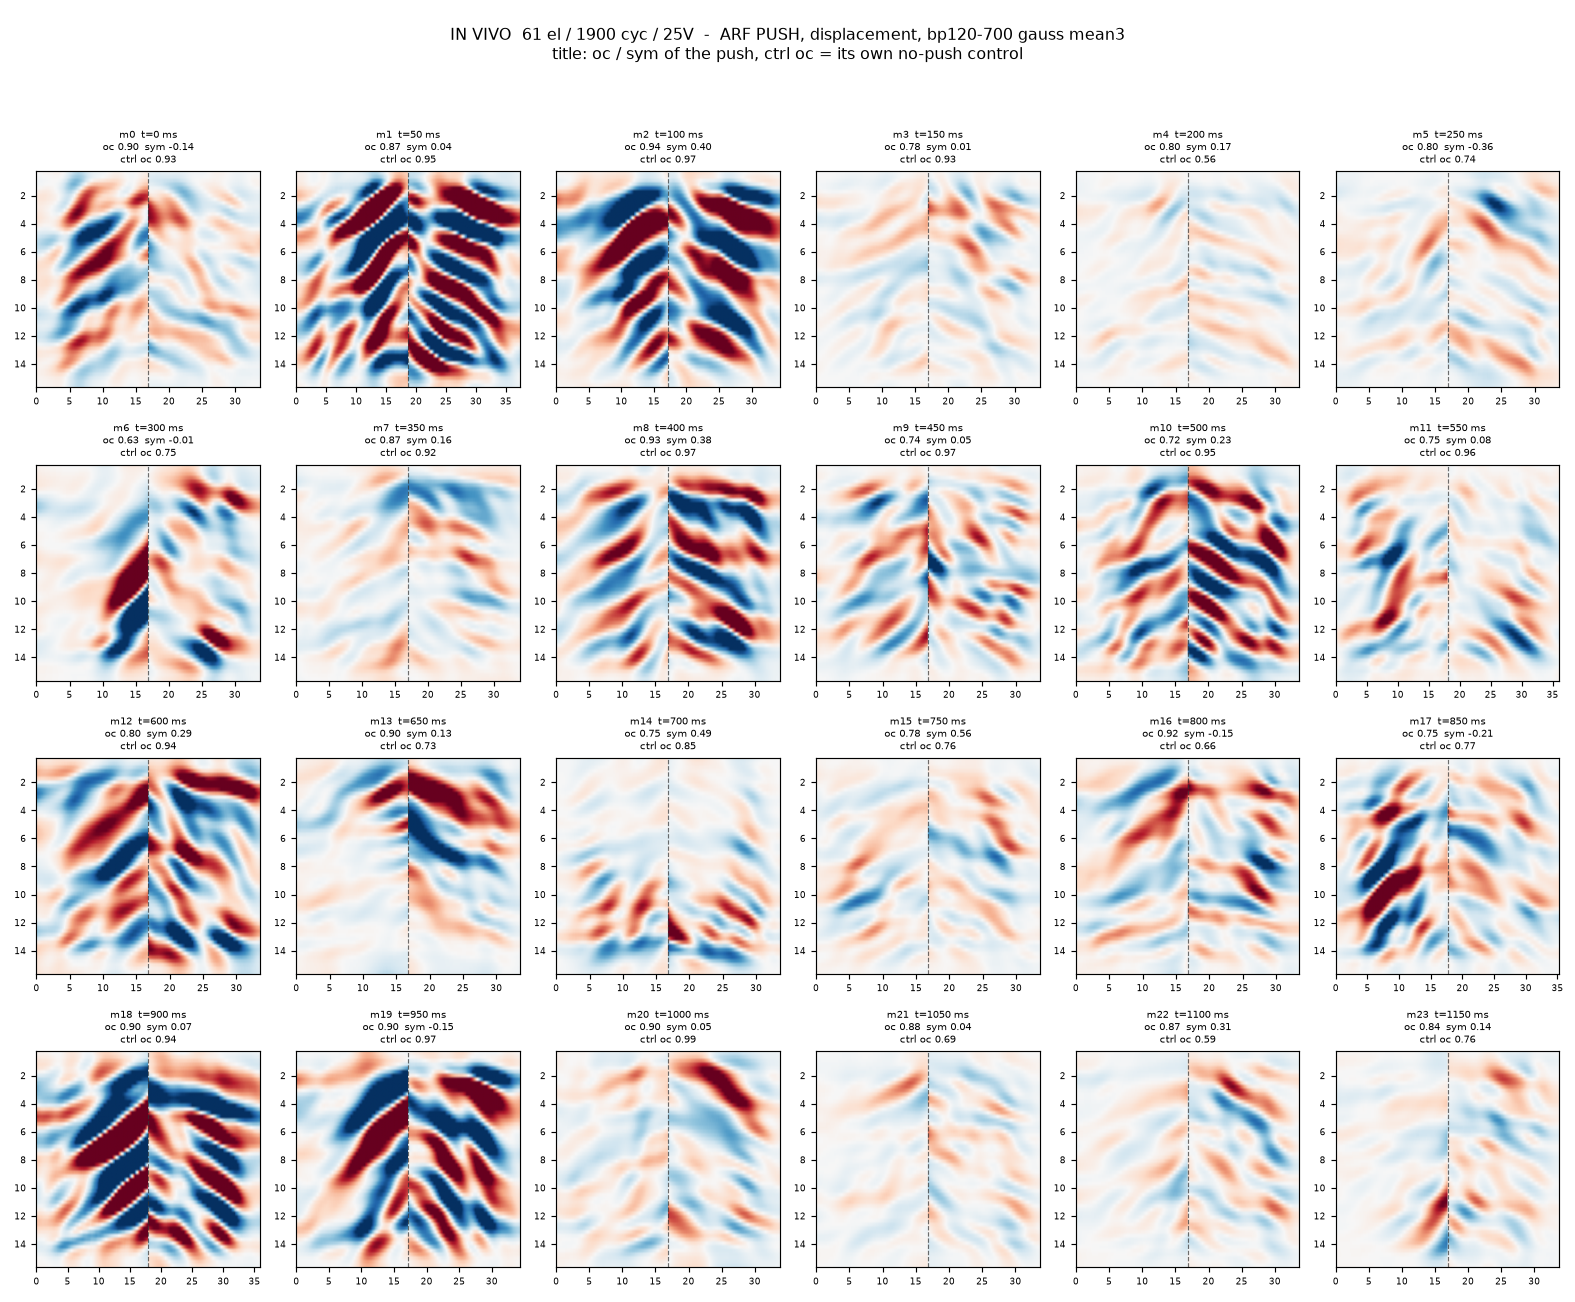
\includegraphics[width=0.95\textwidth]{sweep_invivo_61el_push.png}
\caption{Q4, all 24 pushes of the recommended configuration (61\,el / 1900\,cyc / 25\,V), ARF push,
displacement, in-vivo recipe. \texttt{ctrl oc} is that push's own no-push control. The high-amplitude
crossing diagonals of m1, m2, m8, m18 and m19 are cardiac wall motion --- their controls score
0.94--0.99. The quieter pushes (m4, m5, m14, m15, m21, m22) show weak fans but nothing decisive.}
\label{fig:iv61}
\end{figure}

\subsection{Why the null result is consistent rather than contradictory}
Judged by delivered acoustic output rather than by volts, the two in-vivo acquisitions were
near-equivalent pushes, and neither was the strongest legal option:
\begin{itemize}
  \item \textbf{41\,el / 1500\,cyc / 30\,V}: measured $I_\mathrm{sppa.3}=163$, i.e.\ \emph{under} the
  190 limit --- \SI{2}{\volt} of headroom that was available and not used.
  \item \textbf{61\,el / 1900\,cyc / 25\,V}: measured $I_\mathrm{sppa.3}=220$, \bad{16\,\% over the
  limit} (the legal voltage at 61 elements is \SI{23.1}{\volt}), and on the phantom this
  configuration scores 0.64 against 41\,el\,@\,\SI{32}{\volt}'s 0.76.
  \item On the phantom both sit at a quality of roughly 0.6--0.7, the regime where the V is present but
  soft. In a moving myocardium that margin disappears.
\end{itemize}
So this experiment did not test ``a much stronger push''. It tested two pushes of similar strength, one
of which traded transmit voltage for aperture at roughly constant focal intensity. \caveat{H0 --- the
push-strength hypothesis --- therefore remains untested at the strongest legal setting}, although the
ceiling is now known and it is close: the best legal configuration scores about
$0.76/0.64\approx1.2\times$ the 61-element acquisition and $0.76/0.68\approx1.1\times$ the
41-element one on the phantom --- not an order of magnitude, and not obviously enough to turn a null
result into a positive one.

A second observation cuts against H0 as the \emph{sole} explanation. Across all four in-vivo
acquisitions the no-push controls carry as much energy as the pushes (Figure~\ref{fig:ivsum}, left;
control origin coherence routinely 0.93--0.99). Whatever the push adds, it is small compared with what
the wall is already doing. That is a signal-\emph{contrast} problem, not only a signal-strength problem,
and raising the push alone may not resolve it --- \S\ref{sec:pipeline} takes that seriously.

\paragraph{M-lines.} The results above use the automatic septal M-lines
(\S\ref{sec:problems}), validated in aggregate against 24 hand-drawn lines. Hand-drawn lines for
these two acquisitions are being produced with \texttt{scripts/draw\_invivo\_mlines.py}, which
walks through all 24 pushes per folder with the push focus and the automatic proposal overlaid, and
saves each line as it is drawn. \caveat{Every in-vivo number here should be re-checked once those
exist}; the aggregate validation says the conclusion is unlikely to move, but the per-push scatter
is large enough that individual panels can.

% ======================================================================
\section{Conclusions}\label{sec:conclusions}
% ======================================================================
\begin{enumerate}[label=\textbf{C\arabic*.},leftmargin=2.6em]
  \item \textbf{The pipeline is not the problem.} The report's phantom result reproduces end-to-end
  from the raw IQ (\S\ref{sec:q1}), and the same code recovers a crisp symmetric V from the new
  phantom data at every configuration above $\sim$\SI{30}{\volt}.
  \item \textbf{A silent reconstruction bug cost one round of conclusions} (\S\ref{sec:bug}). The
  buffer-2 receive length is a runtime quantity taken from a constant base config; when the two
  disagree, the B-modes stay perfect and only the tracking data is destroyed. This is a design
  hazard in \texttt{make\_combined\_data.m}, not a one-off, and it is now guarded in code. The
  lesson generalises: \emph{check frame-to-frame speckle correlation before believing any negative
  shear-wave result} --- it took one number to separate ``no wave in the tissue'' from ``no wave in
  the reconstruction''.
  \item \textbf{The 2026-08-07 parameter ranking replicates} on independent data and on two
  different probes (\S\ref{sec:q2}, \S\ref{sec:q3}): more elements and a longer pulse are better
  \emph{at matched transmit voltage}, monotonically, with the aperture the stronger lever.
  \item \textbf{But that comparison answers the wrong question} (\S\ref{sec:isosafety}). The push is
  $I_\mathrm{sppa.3}$-limited, so apertures cannot be compared at fixed voltage --- only one of the
  three 30\,V cells is even legal. At matched, legal acoustic output the ranking reverses and
  \good{41 elements beats 61 and 79} (mirror symmetry 0.76 vs 0.58 vs 0.55 at
  $I_\mathrm{sppa.3}=190$), reproducibly across three datasets and both probes. Physically:
  constraining the spatial-\emph{peak} intensity penalises the tighter focus, because the
  radiation-force impulse depends on the intensity integrated over the focal volume.
  \item \textbf{All three apertures are now measured, and the numbers are lower than the
  extrapolation} (\S\ref{sec:safety}). The 41-element ceiling is \SI{32.0}{\volt}, not the
  \SI{35}{\volt} the old table implied; \bad{the 61\,el / 25\,V in-vivo acquisition was 16\,\% over
  the $I_\mathrm{sppa.3}$ limit}. MI is never the binding limit --- it has reached only 1.5--1.6 at
  each aperture's legal maximum. No firing-to-firing supply sag is measurable, either in the
  hydrophone repeats (1--2\,\% within a capture) or in the shear-wave data ($-1.5\,\%$ from push 0
  to push 9 across 30 configurations).
  \item \textbf{The aperture optimum is near 41 elements, not lower} (\S\ref{sec:trend}). Below
  $\approx$\,27 elements the 50\,V transmit ceiling binds before the safety limit does, so the
  aperture can no longer reach the legal output at all: 21 elements tops out at
  \SI{126}{\watt\per\square\centi\metre} and its measured quality is flat at $\approx0.48$ from 20
  to 30\,V --- the ``not enough acoustic power'' regime. The window \textbf{27--41 elements} is
  untested and is where any remaining gain lives.
  \item \textbf{Neither S5-1 probe is degraded} (\S\ref{sec:q3}). The probe-to-probe difference
  equals the day-to-day repeatability of a single probe (RMS 0.039 vs 0.034 in mirror symmetry).
  That hypothesis is closed.
  \item \textbf{The in-vivo measurement did not improve} (\S\ref{sec:q4}). No configuration --- old
  or new, 41 or 61 elements --- produces a space-time that beats its own no-push control; median
  push-minus-control origin coherence is $-0.05$ to $+0.02$ across all four acquisitions.
  \item \textbf{H0 (push-strength-limited) is neither confirmed nor refuted}, because the experiment
  did not deliver a stronger push: by measured acoustic output the two new configurations were
  equivalent to each other, and one of them was under the limit it could have used while the other
  was over it. What \emph{is} now known is the size of the remaining headroom, and it is small ---
  the best legal configuration scores 1.1--1.2$\times$ what was used, on a phantom, with no cardiac
  motion.
  \item \textbf{A second explanation deserves equal weight.} The no-push controls carry as much
  energy as the pushes (control origin coherence routinely 0.93--0.99). That is a contrast problem
  as much as an amplitude problem, and no achievable push increase closes a gap of that size on its
  own.
\end{enumerate}

% ======================================================================
\section{Recommendation on parameter selection}\label{sec:recommend}
% ======================================================================
\good{Use 41 push elements, 1900 cycles, \SI{32}{\volt}, R-peak triggered.} In detail:

\begin{description}[leftmargin=1.2em,style=nextline]
  \item[Push aperture: 41 elements --- go back down, not up to 61.] At matched, legal acoustic output
  the 41-element push is clearly better (mirror symmetry 0.76 vs 0.58 vs 0.55 for 41/61/79 elements
  at $I_\mathrm{sppa.3}=190$), and this replicates in three independent datasets and both probes.
  The previous 61-element recommendation was derived at matched voltage, before the hydrophone
  campaign established that $I_\mathrm{sppa.3}$ binds.
  \item[Push voltage: \SI{32}{\volt} --- the measured ceiling, not \SI{35}{\volt}.] This is the whole
  point of choosing the smaller aperture: it buys voltage headroom. The direct measurement puts
  $I_\mathrm{sppa.3}$ at exactly 190 and MI at 1.48 there. \caveat{\SI{35}{\volt} is not available}
  --- the measured $I_\mathrm{sppa.3}$ at 35\,V is \SI{230}{\watt\per\square\centi\metre}. Set the
  push TPC profile's \texttt{highVoltageLimit} to 32\,V so it cannot be exceeded by accident.
  \item[Push pulse length: keep 1900 cycles, and longer is worth testing.] It beats 1500 cycles at
  every operating point, costs nothing on MI or $I_\mathrm{sppa}$ (both are peak/pulse-average
  quantities), and the resulting $I_\mathrm{spta.3}$ is only
  \SI{117}{\milli\watt\per\square\centi\metre} at the recommended setting against a
  \SI{720}{\milli\watt\per\square\centi\metre} limit. Even doubling the pulse length again would
  leave a factor $\sim$3 of margin. \caveat{Note} the highest cells of the sweep reach
  \SI{385}{\milli\watt\per\square\centi\metre}, still under Track 3 but approaching the older
  application-specific cardiac figure of \SI{430}{\milli\watt\per\square\centi\metre}; the
  recommended setting is far from both.
  \item[Tracking: keep the R-peak trigger.] It was added for these acquisitions and it works; it makes
  cardiac-phase-resolved comparison possible for the first time, which is worth keeping regardless of
  how the push question resolves.
  \item[Apodization: unchanged (uniform).] Nothing in this campaign bears on it. The earlier
  reasoning --- do not spend force on margin --- now applies to a \emph{smaller} aperture, where there
  is even less reason to taper.
\end{description}

\paragraph{Expected gain, stated honestly.} Against the 41\,el / 1500\,cyc / 30\,V acquisition this
buys 1900 cycles and \SI{2}{\volt}: phantom mirror symmetry $0.59\rightarrow0.76$. Against the
61\,el / 1900\,cyc / 25\,V acquisition it buys $0.64\rightarrow0.76$ \emph{and} brings the
acquisition back inside the $I_\mathrm{sppa.3}$ limit. \caveat{Both are real but modest}, and
neither is obviously large enough to lift the in-vivo push-minus-control contrast off zero.

\paragraph{The one configuration that might do better is untested.} If the measured focal-gain
scaling holds, \textbf{31 elements at $\approx$\,\SI{41}{\volt}} and \textbf{27 elements at
$\approx$\,\SI{50}{\volt}} also reach $I_\mathrm{sppa.3}=190$, but with a larger focal volume than
41 elements, and should therefore be better again. Below 27 elements the transmit ceiling binds and
the output collapses (21 elements reaches only 126). Two phantom acquisitions would settle it.

% ======================================================================
\section{Q5 --- can pushes from two heartbeats be combined?}\label{sec:crossbeat}
% ======================================================================
Averaging repeated pushes at a fixed cardiac phase across beats was proposed as a way to buy SNR
without touching MI or $I_\mathrm{sppa}$ (the $I_\mathrm{spta.3}$ budget has 5.8$\times$ of slack).
The objection to it is practical and decisive: a patient cannot hold their breath for
\SI{20}{\second}, and fixing the phase throws away the one thing active SWE offers over the
natural-wave method --- stiffness \emph{throughout} the cycle rather than at the two valve-closure
events.

The proposal can nevertheless be tested for free, because the acquisition already spans more than
one beat. At $\approx$\,68\,bpm the 24 pushes on a \SI{50}{\milli\second} grid cover
\SI{1.15}{\second} $=$ 1.33 cardiac cycles, so the last pushes repeat the cardiac phase of the
first ones in the \emph{next} beat. The ECG record stored with each acquisition
(\texttt{ECG\_data\_raw}: ECG samples, detected R-peaks, and every Verasonics trigger) fixes the
phase of each push exactly --- and confirms the gating works: push 0 fires
\SI{12}{\milli\second} after the R-peak in both acquisitions.

\begin{table}[h]
\centering\small
\caption{Q5: 13 cross-beat, phase-matched push pairs across the two in-vivo acquisitions.
\texttt{ncc} is the normalised cross-correlation of two space-times; the null is the same quantity
for phase-\emph{mismatched} control pairs within one beat. Push and control correlations are
computed on the \emph{same} \SI{8.1}{\milli\second} window, so the comparison is like-for-like.}
\label{tab:crossbeat}
\begin{tabular}{@{}lcccccc@{}}
\toprule
\textbf{Acquisition} & \textbf{pairs} & \textbf{$\Delta$phase} & \textbf{null} &
\textbf{control--control} & \textbf{push--push} & \textbf{$\Delta$OC single $\rightarrow$ 2-beat} \\
\midrule
41\,el / 1500\,cyc / 30\,V & 6 & \SI{13.9}{\milli\second} & 0.18 & $+0.42$ & $+0.27$ & $-0.013 \rightarrow -0.020$ \\
61\,el / 1900\,cyc / 25\,V & 7 & \SI{6.1}{\milli\second}  & 0.16 & $+0.46$ & $+0.07$ & $-0.028 \rightarrow -0.039$ \\
\bottomrule
\end{tabular}
\end{table}

\begin{figure}[t]
\centering
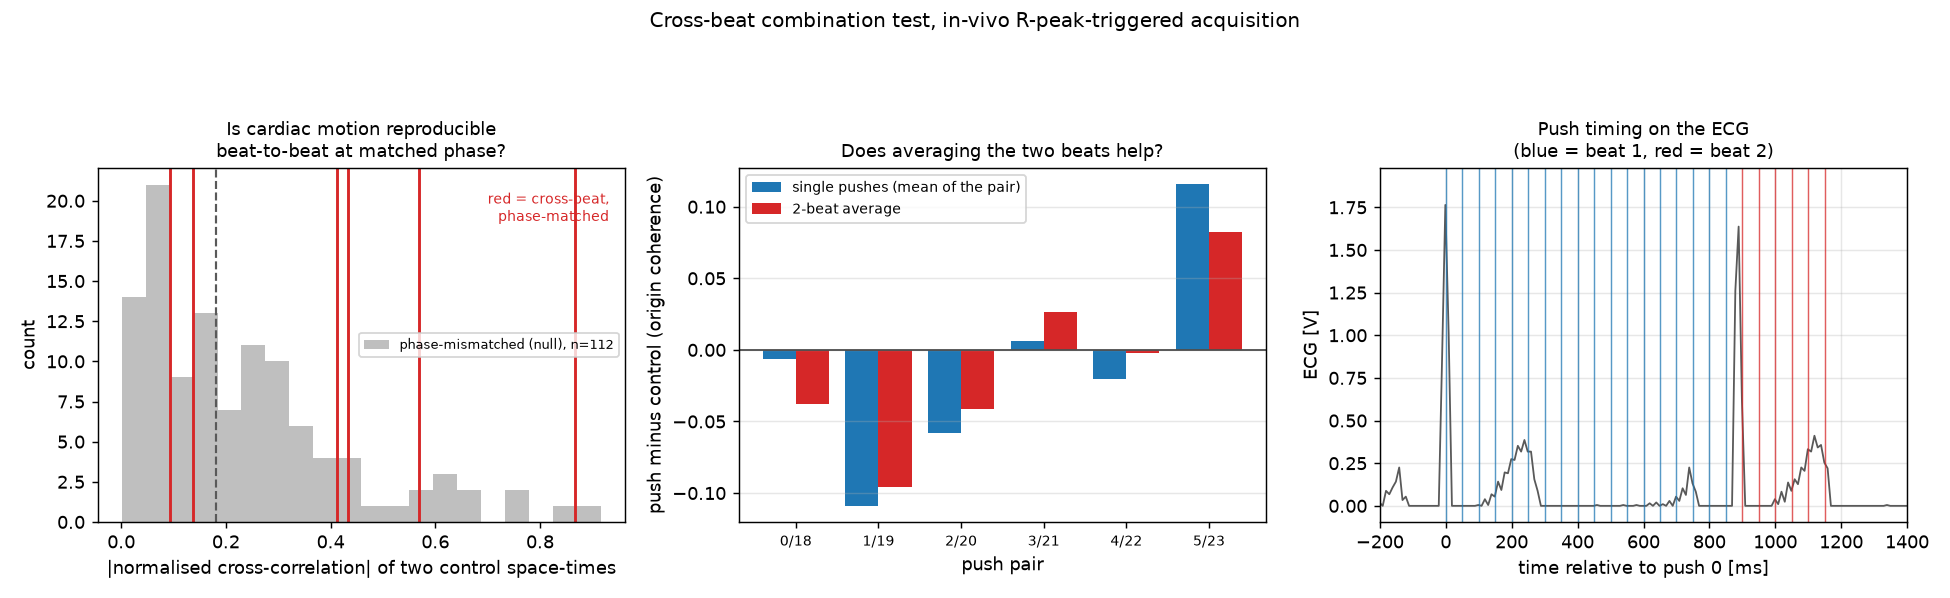
\includegraphics[width=\textwidth]{sweep_crossbeat_summary.png}
\caption{Q5 summary (41-element acquisition). \emph{Left:} cross-correlation of two control
space-times --- grey is the phase-mismatched null, red lines are the cross-beat phase-matched pairs.
\emph{Middle:} push-minus-control contrast for the single pushes versus their 2-beat average.
\emph{Right:} push timing on the ECG, blue for beat 1 and red for beat 2; push 0 fires
\SI{12}{\milli\second} after the R-peak.}
\label{fig:crossbeat}
\end{figure}

Three results, and the second is the important one:

\begin{enumerate}[label=\textbf{\arabic*.}]
  \item \textbf{Cardiac motion is only partially reproducible beat-to-beat at matched phase.}
  Control-to-control correlation is $+0.42$/$+0.46$ against a null of $0.18$/$0.16$ --- above
  chance, but nowhere near the reproducibility a subtraction scheme would need, and enormously
  variable (individual pairs range from $-0.36$ to $+0.89$). Averaging will not suppress it, and
  subtracting it would not cancel it either.
  \item \bad{The push response is \emph{less} reproducible than the cardiac motion.} On the same
  window, push-to-push correlation is $+0.27$ and $+0.07$, \emph{below} the control-to-control
  figures. If a genuine ARF wave were present it would be the deterministic, push-locked part of the
  signal, and two pushes at the same cardiac phase would agree \emph{better} than their pre-push
  references do. They agree worse. \good{This is an independent line of evidence, separate from the
  push-minus-control test of \S\ref{sec:q4}, that there is no consistent ARF wave in this data} ---
  what occupies the push window behaves like noise.
  \item \textbf{Averaging the two beats does not help.} The median push-minus-control contrast moves
  from $-0.013$ to $-0.020$ (41\,el) and $-0.028$ to $-0.039$ (61\,el): slightly worse in both.
  Individual pairs scatter $\pm0.05$ with no trend.
\end{enumerate}

\caveat{Power caveat.} Two beats can buy at most $\sqrt{2}=1.41\times$ even under ideal conditions,
$n=13$ pairs is small, and the phase match is imperfect (\SIrange{6}{14}{\milli\second}). This does
not formally exclude a gain at $N=20$. But combined with result 2 it removes the reason to expect
one: averaging helps only if there is something deterministic to average, and the data says there
is not. \good{The beat-combination proposal is therefore withdrawn}; what survives from
\S\ref{sec:pipeline} is the reference-model and detector work, which does not assume repeatability
across beats.

\begin{figure}[p]
\centering
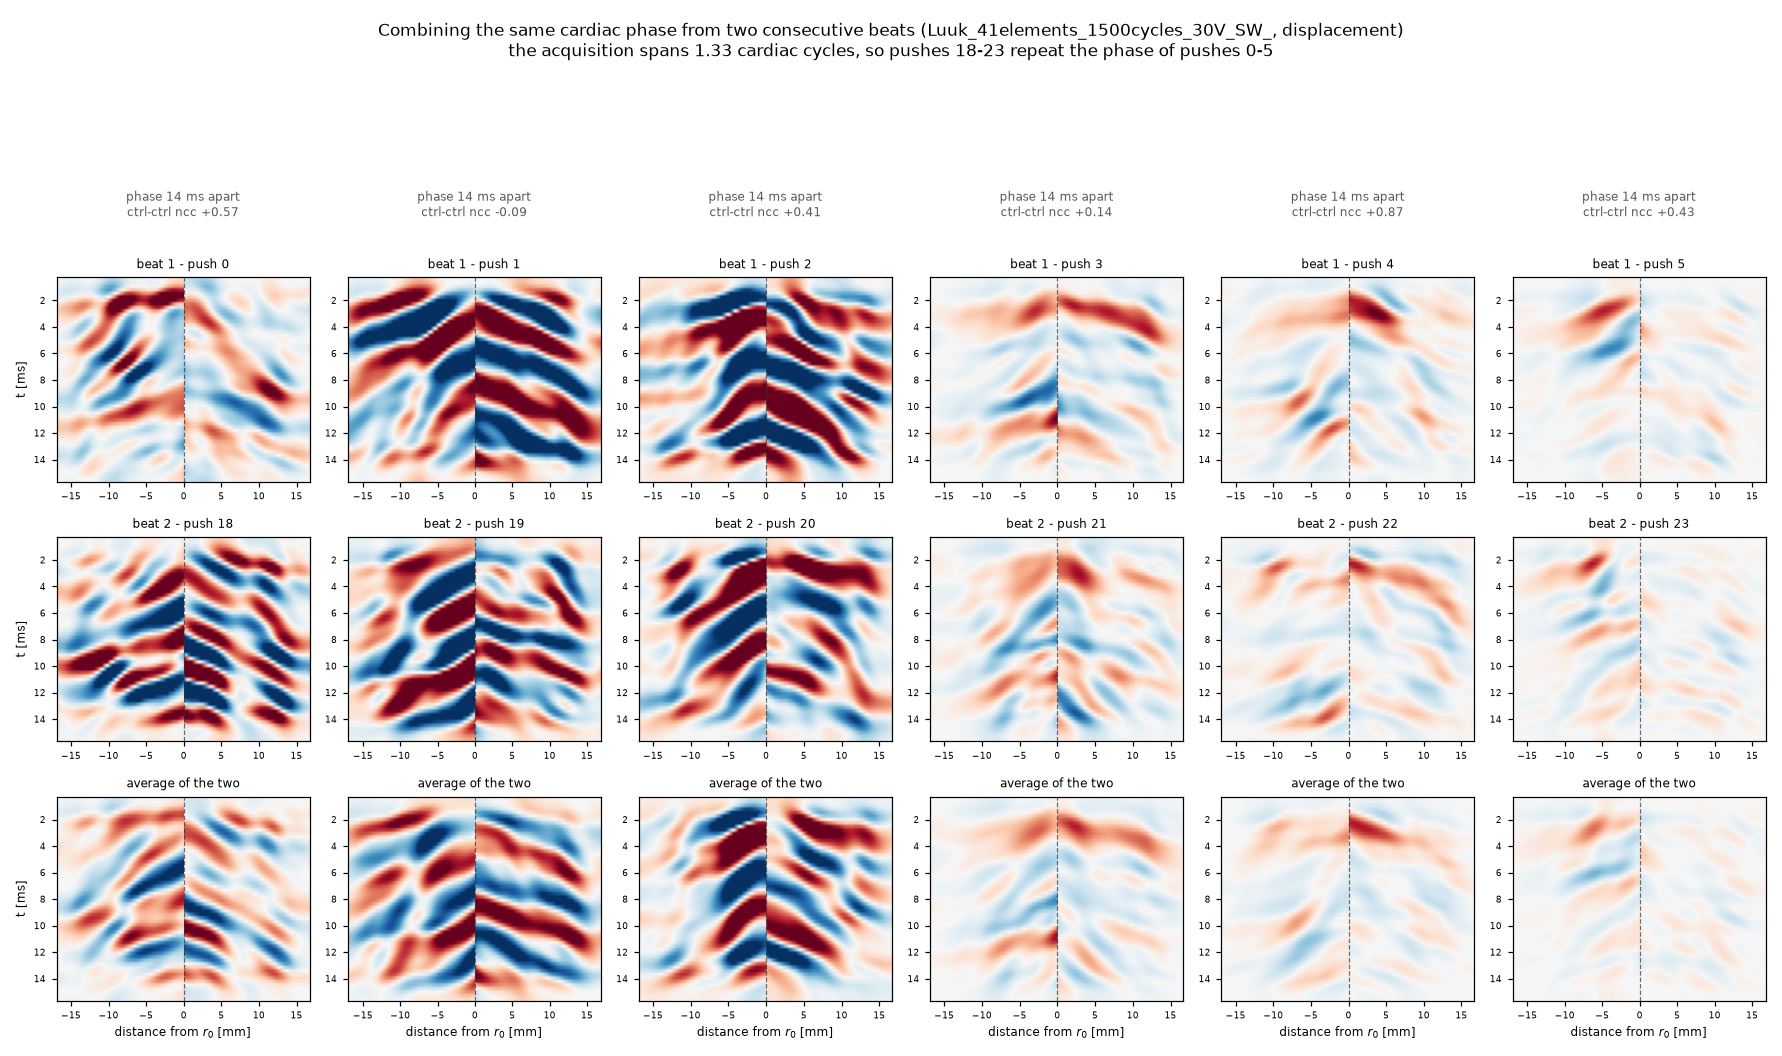
\includegraphics[width=0.95\textwidth]{sweep_crossbeat_pushes.png}
\caption{Q5, the six phase-matched pairs of the 41-element acquisition: beat 1, beat 2, and their
average. The early-systolic pairs (pushes 0--2, \SIrange{12}{112}{\milli\second} after the R-peak)
are dominated by high-amplitude crossing diagonals that survive averaging unchanged --- the
reproducible part of the cardiac motion. The quieter late pairs average to nothing in particular. No
pair produces a symmetric V that either member lacks.}
\label{fig:crossbeatpushes}
\end{figure}

% ======================================================================
\section{Does the ``contrast problem'' mean the pipeline needs work?}\label{sec:pipeline}
% ======================================================================
Partly --- but the honest answer is that the pipeline is not where the biggest remaining factor is,
and it is worth being precise about which parts of it are and are not exhausted.

\paragraph{What is already exhausted.} The \emph{extraction} half has had a very large search:
$\sim$700 recipes $\times$ 8 voltages $\times$ 3 quantities on the phantom, a 52-push sweep on the
Caenen pig data, and a 700-recipe per-lobe scan on the in-vivo 40\,V set. That search converged on a
stable family (Loupas $\cdot$ relative-to-reference $\cdot$ temporal band-pass $\cdot$
outward-directional $\cdot$ moving-mean $\cdot$ 7--9 offsets) and established that the estimator
barely matters, that a fine-grid RF cross-correlation is \emph{worse} at low SNR, and that a finer
beamforming grid does not help. \good{Trying more variations of the same filter chain is unlikely to
pay.} The same recipe recovers a clean V from the phantom and from the Caenen pig data, so it is not
that the pipeline cannot see a cardiac ARF wave.

\paragraph{What is not exhausted, and is genuinely a pipeline question.} The failure mode in vivo is
specific: the no-push control is as strong as the push. That is a \emph{separation} problem between
two signals occupying the same band, not a denoising problem, and the pipeline currently attacks it
with band-pass plus an outward-directional filter --- both of which are blind to the distinction.
Three directions are open:
\begin{itemize}
  \item \textbf{Use the control, don't just plot it.} At present the no-push control is a diagnostic
  drawn beside the push. The pre-push reference block is a \emph{measurement of the cardiac motion
  field} for that push, at that phase, in that beat. Fitting a motion model on the reference and
  extrapolating it across the push window (the report's \texttt{reference poly-extrapolation} /
  \texttt{adaptive high-pass} family) is the natural use of it. \caveat{This is exactly where the
  data-leakage trap lives}: reference-subspace projection and SVD-on-displacement were both shown to
  \emph{fabricate} a symmetric V from pure cardiac motion. Any method in this family has to be
  validated on a held-out split reference before it is believed.
  \item \caveat{Exploit the R-peak trigger --- proposed here, tested in \S\ref{sec:crossbeat}, and
  it fails.} The idea was that with gating the same cardiac phase is sampled repeatedly, so
  beat-to-beat averaging and phase-matched subtraction become possible, with the cardiac motion the
  part that repeats and the ARF response fixed relative to the push. \bad{Neither half holds:} the
  cardiac motion repeats only weakly ($+0.42$ against a $0.18$ null), and the push response repeats
  \emph{less} well than the cardiac motion does. Recorded here because it was a reasonable idea that
  the existing data was able to kill outright, at no acquisition cost.
  \item \textbf{Detect rather than image.} All current metrics score a picture. A matched-filter or
  model-based detector --- fit an outward-propagating cylindrical wave with an unknown speed and
  amplitude and test its significance against the control --- would use the known push time and
  origin far more efficiently than a band-pass plus a symmetry score, and would give a $p$-value
  instead of a judgement call.
\end{itemize}

\paragraph{But keep the ordering right.} These are worth doing, and they are cheap compared with
scanner time. They are still second in line behind the acquisition, for one reason: on the phantom,
with \emph{no} cardiac motion at all, the best legal configuration only reaches a mirror symmetry of
0.76, and the recipe that produces it is the same one that fails in vivo. If the push were strong
enough, the current pipeline would already show something.

\paragraph{And after \S\ref{sec:crossbeat}, be honest about which half is broken.} The
cross-beat test found that the push windows are \emph{less} reproducible across matched-phase beats
than the pre-push references are. A processing method can separate two signals; it cannot recover
one that is not there. \bad{On the present evidence the in-vivo push windows contain no consistent
ARF response at all}, which makes this a signal-generation problem first and a processing problem
second. The reference-model and detector work in this section is worth doing because it will make
the \emph{next} acquisition easier to judge --- not because it is likely to extract a wave from
these recordings.

% ======================================================================
\section{Remaining next steps}\label{sec:next}
% ======================================================================
\begin{enumerate}[label=\textbf{\arabic*.}]
  \item \textbf{Acquire the recommended in-vivo configuration} --- 41\,el / 1900\,cyc /
  \SI{32}{\volt}, R-peak triggered --- and re-run \texttt{scripts/task4b\_config\_contrast.py}. This
  is the actual test of H0, which has still not been performed. Raise the push TPC profile's
  \texttt{highVoltageLimit} to exactly 32\,V first.
  \item \textbf{Phantom: acquire 31 elements at \SI{41}{\volt} and 27 elements at \SI{50}{\volt}}
  (1900 cycles), the two configurations that should reach the full legal output with a larger focal
  volume than 41 elements. Together with the existing 21/41/61/79-element points this closes the
  aperture curve. Ideally add a hydrophone point for whichever wins, since their output is currently
  scaled rather than measured.
  \item \textbf{Finish the hand-drawn in-vivo M-lines} (\texttt{scripts/draw\_invivo\_mlines.py})
  and re-run Q4. The \SI{2.4}{\milli\metre} mean separation between automatic and manual lines is of
  the same order as the septal wall thickness, so single-push readings need them.
  \item \textbf{Hydrophone follow-ups.} Resolve the two 79-element datasets by re-measuring at a
  deliberately re-peaked position with the 3-firing protocol (the peak-optimised and repeats sets
  differ by 1.6$\times$; session A says the former is right, but it should not rest on that alone).
  Still open from the safety notes: a transient thermal (TI) estimate for the \SI{1.2}{\second}
  burst, and the L12-3 table.
  \item \textbf{Verify the delivered transmit voltage} at the top of a sweep, given the 0.6\,A vs
  0.5\,A supply warning. The push-index analysis (Figure~\ref{fig:pushidx}) and the hydrophone
  repeats both say there is no sag, so this is now a confirmation rather than an open risk --- a
  current probe at 40\,V would close it.
  \item \textbf{Pipeline work, in the order of \S\ref{sec:pipeline}}: reference-model motion removal
  with held-out validation, and a model-based detector with a significance test instead of a visual
  score. \emph{Not} beat-to-beat combination --- \S\ref{sec:crossbeat} tested that on the existing
  data and it does not work.
  \item \textbf{Fold this into the main report.} \texttt{report/main.tex} \S9 recommends 61 elements
  and should be amended with the iso-output argument and the measured safety table.
\end{enumerate}

% ======================================================================
\appendix
\section{Code, outputs and how to reproduce}
% ======================================================================
All new code is in \texttt{shearWaveProcessing}, uncommitted at the time of writing.

\begin{longtable}{@{}p{6.0cm}p{10.2cm}@{}}
\toprule
\textbf{File} & \textbf{Purpose} \\
\midrule
\endhead
\texttt{scripts/swe\_lib.py} & Shared helpers: the two recipes, space-times built straight from
buffer-2 IQ, the no-push control, and the scoring wrappers. \\
\texttt{scripts/fix\_buffer2\_receive.py} & The receive-layout repair of \S\ref{sec:bug} (standalone,
with a \texttt{--check} dry run). \\
\texttt{src/swp/acquisition/combined.py} & \texttt{repair\_buffer2\_receive()} folded into
\texttt{ensure\_combined\_data} so the check runs on every build. \\
\texttt{scripts/batch\_prepare.py} & Build \texttt{CombinedData.mat} $\rightarrow$ repair $\rightarrow$
beamform, for every folder under one or more roots. \\
\texttt{scripts/beamform\_sw\_only.py} & Beamform only buffers 2 and 5 (in vivo, buffers 1/3/4/6 are
large and unused here). \\
\texttt{scripts/task1\_repro\_voltage.py} & Figure~\ref{fig:q1}. \\
\texttt{scripts/task2\_element\_cycle\_grid.py} & Figures~\ref{fig:grid1900}, \ref{fig:grid1500},
\ref{fig:scores} and the scores CSV. \\
\texttt{scripts/task2b\_iso\_safety.py} & Figure~\ref{fig:iso} and Table~\ref{tab:iso}. \\
\texttt{scripts/task3\_probe\_compare.py} & Figures~\ref{fig:probe}, \ref{fig:bmode} and the paired
grids. \\
\texttt{scripts/task4\_invivo\_compare.py} & Figures~\ref{fig:ivsum}, \ref{fig:ivbest}, \ref{fig:iv61}
and the in-vivo scores CSV. \\
\texttt{scripts/task4b\_config\_contrast.py} & Figure~\ref{fig:ivcontrast} and Table~\ref{tab:invivo}. \\
\texttt{scripts/auto\_mline.py} & Automatic septal M-line proposal (writes the standard
\texttt{.npz}). \\
\texttt{scripts/draw\_invivo\_mlines.py} & Hand-draw the septal M-line for every in-vivo push;
resumable, saves as it goes, shows the push focus and the automatic proposal as a guide. \\
\texttt{scripts/aperture\_trend.py} & \S\ref{sec:trend}: the 21-element arm, the focal-gain
exponent, and the legal reach of each aperture (Figure~\ref{fig:trend}). \\
\texttt{scripts/push\_index\_trend.py} & \S\ref{sec:safety}: wave quality vs push index within the
burst, the supply-sag check (Figure~\ref{fig:pushidx}). \\
\texttt{scripts/swp\_ecg.py} & Parse the stored ECG / trigger record; map each push to its
cardiac phase; find phase-matched pairs across beats. Reads the runtime \texttt{.mat}, or the
merged \texttt{CombinedData.mat} when that file was lost. \\
\texttt{scripts/task5\_cross\_beat.py} & \S\ref{sec:crossbeat}: the cross-beat combination
test (Figures~\ref{fig:crossbeat}, \ref{fig:crossbeatpushes}, Table~\ref{tab:crossbeat}). \\
\texttt{SWI/Mechanical index/hydrophone\_analysis/SafetyTableAll.m} & \S\ref{sec:safety}: all
hydrophone sessions on one set of conventions; writes \texttt{safety\_table\_all.csv},
\texttt{safety\_maxvoltage.csv} and Figure~\ref{fig:safety}. Supersedes \texttt{SafetyTable.m}
(session A only) and \texttt{CorrectedMaxVoltage.m} (session B only). \\
\texttt{scripts/validate\_auto\_mline.py} & Figure~\ref{fig:mline}. \\
\texttt{src/swp/acquisition/matlab/make\_combined\_from\_workspace.m} & Rebuild a
\texttt{CombinedData.mat} from a session workspace dump (used for the 61-element in-vivo folder). \\
\bottomrule
\end{longtable}

\paragraph{Outputs.} Figures and CSVs are written to an \texttt{analysis/} folder beside each dataset:
the 2026-08-17 folder also has an \texttt{analysis/README.md} recording the bug and the repair.

\paragraph{Reproduction.} In the \texttt{zea} environment
(\texttt{KERAS\_BACKEND=torch}), through short directory junctions:
\begin{verbatim}
python scripts/batch_prepare.py --roots D:/swp_ph17 D:/swp_tue D:/swp_mumc
python scripts/beamform_sw_only.py <invivo folder> ... --overwrite
python scripts/auto_mline.py <invivo folder> --x-span-mm 34 --order 1 --save
python scripts/task1_repro_voltage.py    --root D:/swp_v04/Phantom --out <fig>
python scripts/task2_element_cycle_grid.py --root D:/swp_ph17 --outdir <dir>
python scripts/task2b_iso_safety.py      --csv <scores csv> --out <fig>
python scripts/task3_probe_compare.py    --tue D:/swp_tue --mumc D:/swp_mumc --outdir <dir>
python scripts/task4_invivo_compare.py   --root D:/swp_iv --outdir <dir>
python scripts/task4b_config_contrast.py --folders <f...> --labels <l...> --out <fig>
\end{verbatim}
Total re-processing cost: about 100 folders, $\approx$\,\SI{90}{\second} each, run as two parallel
workers.

\paragraph{Build.} No LaTeX toolchain is installed on the acquisition machine. Compile on Overleaf by
uploading the \texttt{report/} folder, or locally with \texttt{latexmk -pdf acquisition\_sweep\_log.tex}.

\end{document}
